\chapter{Ergebnisse}

= LÄNGSTES/AUSFÜHRLICHSTES KAPITEL!!!

Für jedes Unterkapitel gilt: 
> Erst allgemeines Vorgehen/Methodik definieren
> Danach spezifisch für jeden Browser: Unterschied zwischen Snapshot-Zeitpunkten, insb. zwischen Live- und Dead-Forensik

\section{Firefox}

\subsection*{White-Box Analyse/Common Locations}

Schreiboperationen mit Process Monitor verfolgen:

Im Anhang: Tabelle mit allen geschriebenen Dateien (markiert, wenn nicht mehr wiederherstellbar + markiert, wenn Datei "verändert" (siehe oben: temp, WAL))

Aux-Dateien, welche nicht mehr vorhanden waren, aber dafür "richtige" Dateien:
	- % *\datareporting\glean\db\data.safe
	- % *\datareporting\archived\2023-05\1683405837882.9102466b-e465-4ecb-810f-74ae90c64c63.new-profile.jsonlz4
	- % *datareporting\archived\2023-05\1683405837905.86f4c992-6329-415b-8c29-911a2d4b7f9d.event.jsonlz4
	- % *datareporting\archived\2023-05\1683405837939.abf8b065-41a4-4e94-a044-1cead61e396a.main.jsonlz4
	- % *sessionstore-backups\recovery.jsonlz4
	- % *xulstore.json

Ergebnis: Tabelle mit wiederherstellbaren Dateien: Logfile 1 vs. Logfile 2 + Tool mit dem Datei untersucht wurde
- Dateien, die in beiden Logfiles nicht wiederherstellbar 
\begin{figure}[h!]
	\resizebox{\linewidth}{!}{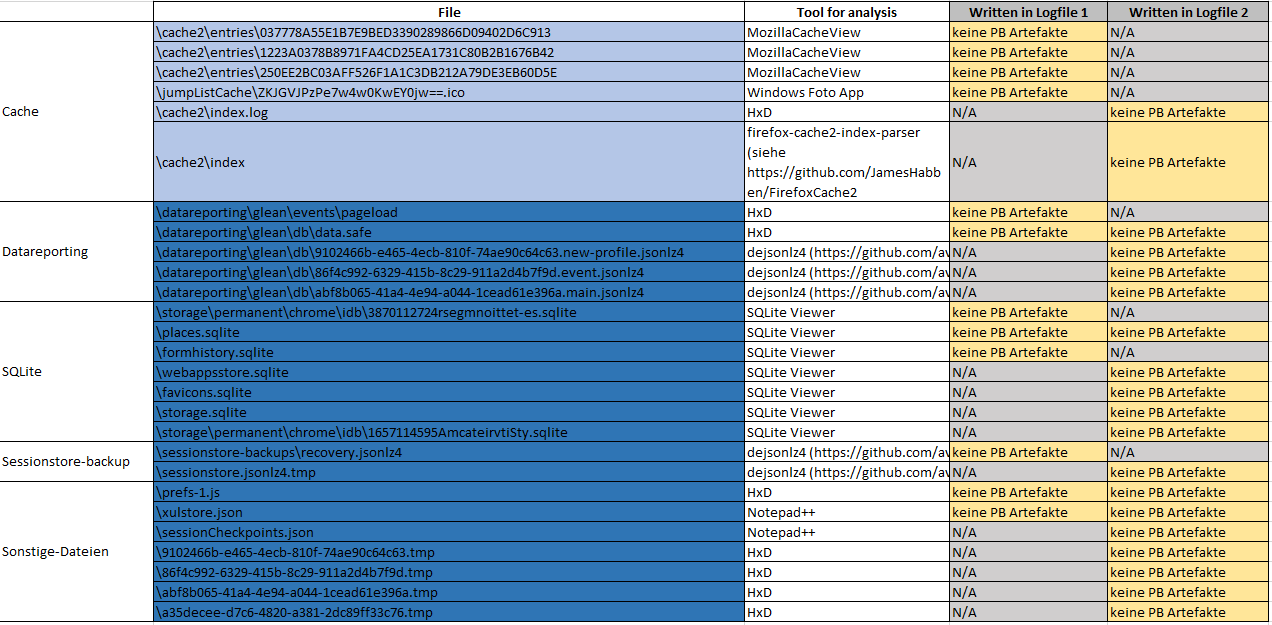
\includegraphics{bilder/firefox-tabelle-logfile1vlogfile2-reduced.png}}
%	\label{...}
	\caption{Tabelle mit wiederherstellbaren Dateien: Logfile 1 vs. Logfile 2}
\end{figure}

Allgemein: Artefakte in zwei "Common Pfaden"
-	(Local) %C:\Users\Forensik\AppData\Local\Mozilla\Firefox\Profiles\<Profile>.default-release\
-	(Roaming) %C:\Users\Forensik\AppData\Roaming\Mozilla\Firefox\Profiles\<Profile>.default-release\

Kategorien der Logs:
- Cache: 
	Logfile 1:
		> % \cache2\entries\037778A55E1B7E9BED3390289866D09402D6C913 (Local)
		> % \cache2\entries\1223A0378B8971FA4CD25EA1731C80B2B1676B42 (Local)
		> % \cache2\entries\250EE2BC03AFF526F1A1C3DB212A79DE3EB60D5E (Local)
		Analyse:
			- Tool: MozillaCacheView
			- TODO: Screenshot
		> % \jumpListCache\ZKJGVJPzPe7w4w0KwEY0jw==.ico (Local)
			- Tool: Windows Foto App
			- Enthält kleines "m" Icon
	Logfile 2:
		> % \cache2\index (Local)
		> % \cache2\index.log (Local)
		Analyse:
			- Tool: siehe Github und HxD
- datareporting:
	Logfile 1:
		> % \datareporting\glean\events\pageload (Roaming)
		> % \datareporting\glean\db\data.safe (Roaming)	
		Analyse:
			- Tool: HxD
			- keine PB Artefakte
	Logfile 2:
		*> % \datareporting\glean\db\data.safe (Roaming)
		> %  \datareporting\glean\db\9102466b-e465-4ecb-810f-74ae90c64c63.new-profile.jsonlz4 (Roaming)
		> % \datareporting\glean\db\86f4c992-6329-415b-8c29-911a2d4b7f9d.event.jsonlz4 (Roaming)
		> % \datareporting\glean\db\abf8b065-41a4-4e94-a044-1cead61e396a.main.jsonlz4 (Roaming)
		Analyse:
			- TODO: Definition glean
			- jsonlz4 Dateien (TODO: Definition) mit dejsonlz4 dekomprimiert (Quelle Github)
			- Dateien enthalten Systeminformationen im Json-Format (Screenshot?)
			- keine PB Artefakte
- Sessionstore-Backup:
	Logfile 1:
		> % \sessionstore-backups\recovery.jsonlz4 (Roaming)
		Analyse:
			- TODO: Definition sessionstore-backup = Datei, die Backup von Sitzungsdaten enthält
			- jsolz4 Datei in sessionstore-backup lassen sich mit Online-Tool parsen (https://www.jeffersonscher.com/ffu/scrounger.html)
			- Ergebnise: 
				Tab 1:  Willkommen bei Firefox [6.5.2023, 22:25:06, about:welcome;
				Tab 2:  Firefox Datenschutzhinweis — Mozilla [6.5.2023, 22:24:59], % https://www.mozilla.org/de/privacy/firefox/
			- Sind Seiten, die sich automatisch geöffnet haben, nachdem Firefox zum ersten Mal geöffnet wurde
			- keine PB Artefakte
	Logfile 2:
		> % \sessionstore.jsonlz4
		Analyse:
			- Lässt sich nicht mit Online-Tool aus Logfile 1 parsen
			- Stattdessen: dejsonlz4, danach Notepad++ mit JSON Plugin
			- Ergebnis: image-Eintrag als base64 entdeckt, in PNG umgewandelt (https://base64.guru/converter/decode/image), mit Windows Foto-App: "m" Icon (Mozilla-Logo)
- Sonstige Dateien:
	Logfile 1:
		> % \prefs-1.js
		> % \xulstore.json			
	Logfile 2:
		*> % \prefs-1.js (Roaming)
		*> % \xulstore.json (Roaming)
		> % \sessionCheckpoints.json (Roaming)
		> % \9102466b-e465-4ecb-810f-74ae90c64c63.tmp (Roaming)
		> % \86f4c992-6329-415b-8c29-911a2d4b7f9d.tmp (Roaming)
		> % \abf8b065-41a4-4e94-a044-1cead61e396a.tmp (Roaming)
		> % \a35decee-d7c6-4820-a381-2dc89ff33c76.tmp (Roaming)
	Analyse:
		- Weder JSON-Dateien (Notepad++) noch .tmp Dateien (HxD) enthalten PB Artefakte
		
- SQLite: (TODO: Abgleich mit Diffs-Exceltabelle, ob wirklich nur in places.sqlite geschrieben wurde)
	Dateien haben Sonderstellung:
		- Diese DBs dienen zur Verwaltung und Speicherung sämtlicher Browser Artefakte, insb. der Browser Historie
		- Aus diesem Grund: Dateien intensiver betrachtet
	Siehe Kapitel Methodik:
		> Entwicklung von Dateiinhalt in allen Snapshots (1, 2, 3 und 4) betrachtet
		> Für jeden Snapshot: 
			- SQLite-Datei extrahiert und mit SQLite-Datei aus vorherigem Snapshot verglichen
			- Untersuchung der SQLite-Dateien mit SQLite-Viewer (GUI-Tools)
			- Wenn zu SQLite-Datei WAL-Datei existiert: mit sqlite3 Kommandozeilentool PRAGMA wal\_checkpoint durchgeführt, danach neue SQLite-Datei mit ursprünglicher SQLite-Datei verglichen
		> Dabei gibt es drei Zustände: 
			- leere Datei
			- neuer (nicht-leerer) Inhalt
			- gleichbleibender Inhalt
	Mit Process Monitor Logfiles festgestellt, dass in folgende SQLite-DBs geschrieben: 
		(TODO: Tabelle mit Spalten: Dateiname, Zweck)
			Dateiename:							Zweck:
		- places.sqlite 						Browsing Historie
		- cookies.sqlite						Speichert Webseiten-Cookies
		- storage.sqlite						Speicher für Webseiten
		- favicons.sqlite						Speichert Icons für Lesezeichen
		- webappsstore.sqlite					Speicher für Webseiten
		- formhistory.sqlite					???
		- 1657114595AmcateirvtiSty.sqlite		> IndexedDB-Dateien, sind DBs, die von besuchten Webseiten
												angelegt werden % (https://www.reddit.com/r/firefox/comments/dri650/what_are_the_idb_files_in_the_permanent_storage/)
												> Im Chrome-Ordner: "the databases in the chrome subfolder relate to various pieces of integrated firefox functionality (content for the new tab page, blocklists, shield/normandy, remote settings, push api, ...)"
												> Enthalten eigentlich URL im Dateinamen
												> TODO: können geparsed werden: % https://stackoverflow.com/a/59923297/18037004
												"Activity Stream for Firefox is a collection of all the things you do in the browser that you care about displayed in a rich and meaningful way" 
												%https://wiki.mozilla.org/Firefox/Activity_Stream
												--> DB enthält keine Browsing Artefakte
		- 3870112724rsegmnoittet-es.sqlite		???
		
	Ergebnisse:
		\begin{figure}[h!]
			\centerline{\resizebox{\linewidth}{!}{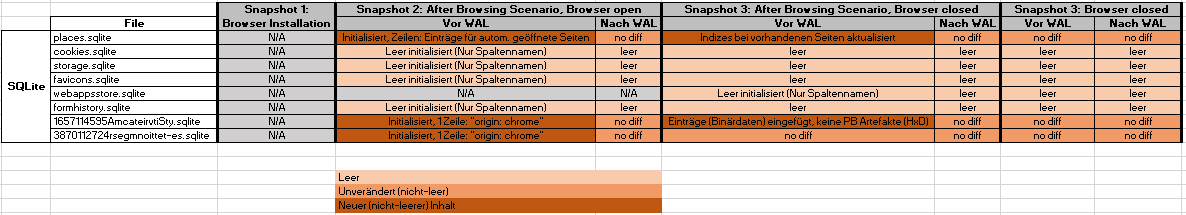
\includegraphics{bilder/firefox-sqlite-table.png}}}
			\label{chart:final-criteria}  
			\caption{Comparison of found PB artifacts between RAM Dumps}
		\end{figure}
		> Nach Browser-Installation noch keine SQLite-Datei angelegt (Snapshot 1)
		> Während Browsing Szenario alle DBs Initialisiert, außer "webappsstore.sqlite" (Snapshot 2)
			- Dabei wurden in places.sqlite die Seiten geschrieben, die sich automatisch nach Browserstart im public Modus geöffnet haben (Datenschutzhinweise zu Firefox)
			- Restliche Dateien ohne Inhalt, nur Spaltennamen
			- Nach WAL Checkpoints bleiben Dateien unverändert
		> Nach Schließen des Browsers (Snapshot 3)
			- in places.sqlite: Indizes bei eingetragenen Seiten aktualisiert
			- 1657114595AmcateirvtiSty.sqlite erhielt BLOB Eintrag, in HxD keine Muster erkennbar
			- webappsstore.sqlite: leer initialisiert, nur Spaltennamen
			- restliche Dateien unverändert
			- nach WAL Checkpoints bleiben Dateien unverändert
		> Nach herunterfahren der VM (Snapshot 4)
			- Alle Dateien unverändert, auch nach WAL Checkpoint
	
- Zusammenfassung: in keiner Datei PB Artefakte


Quantitativ: (Diagramme)		
	> Balkendiagramm: Für jede Logfilekategorie: Anzahl Schreiboperationen Logfile 1 vs Logfile 2
	\begin{figure}[h!]
		\centerline{\resizebox{\linewidth}{!}{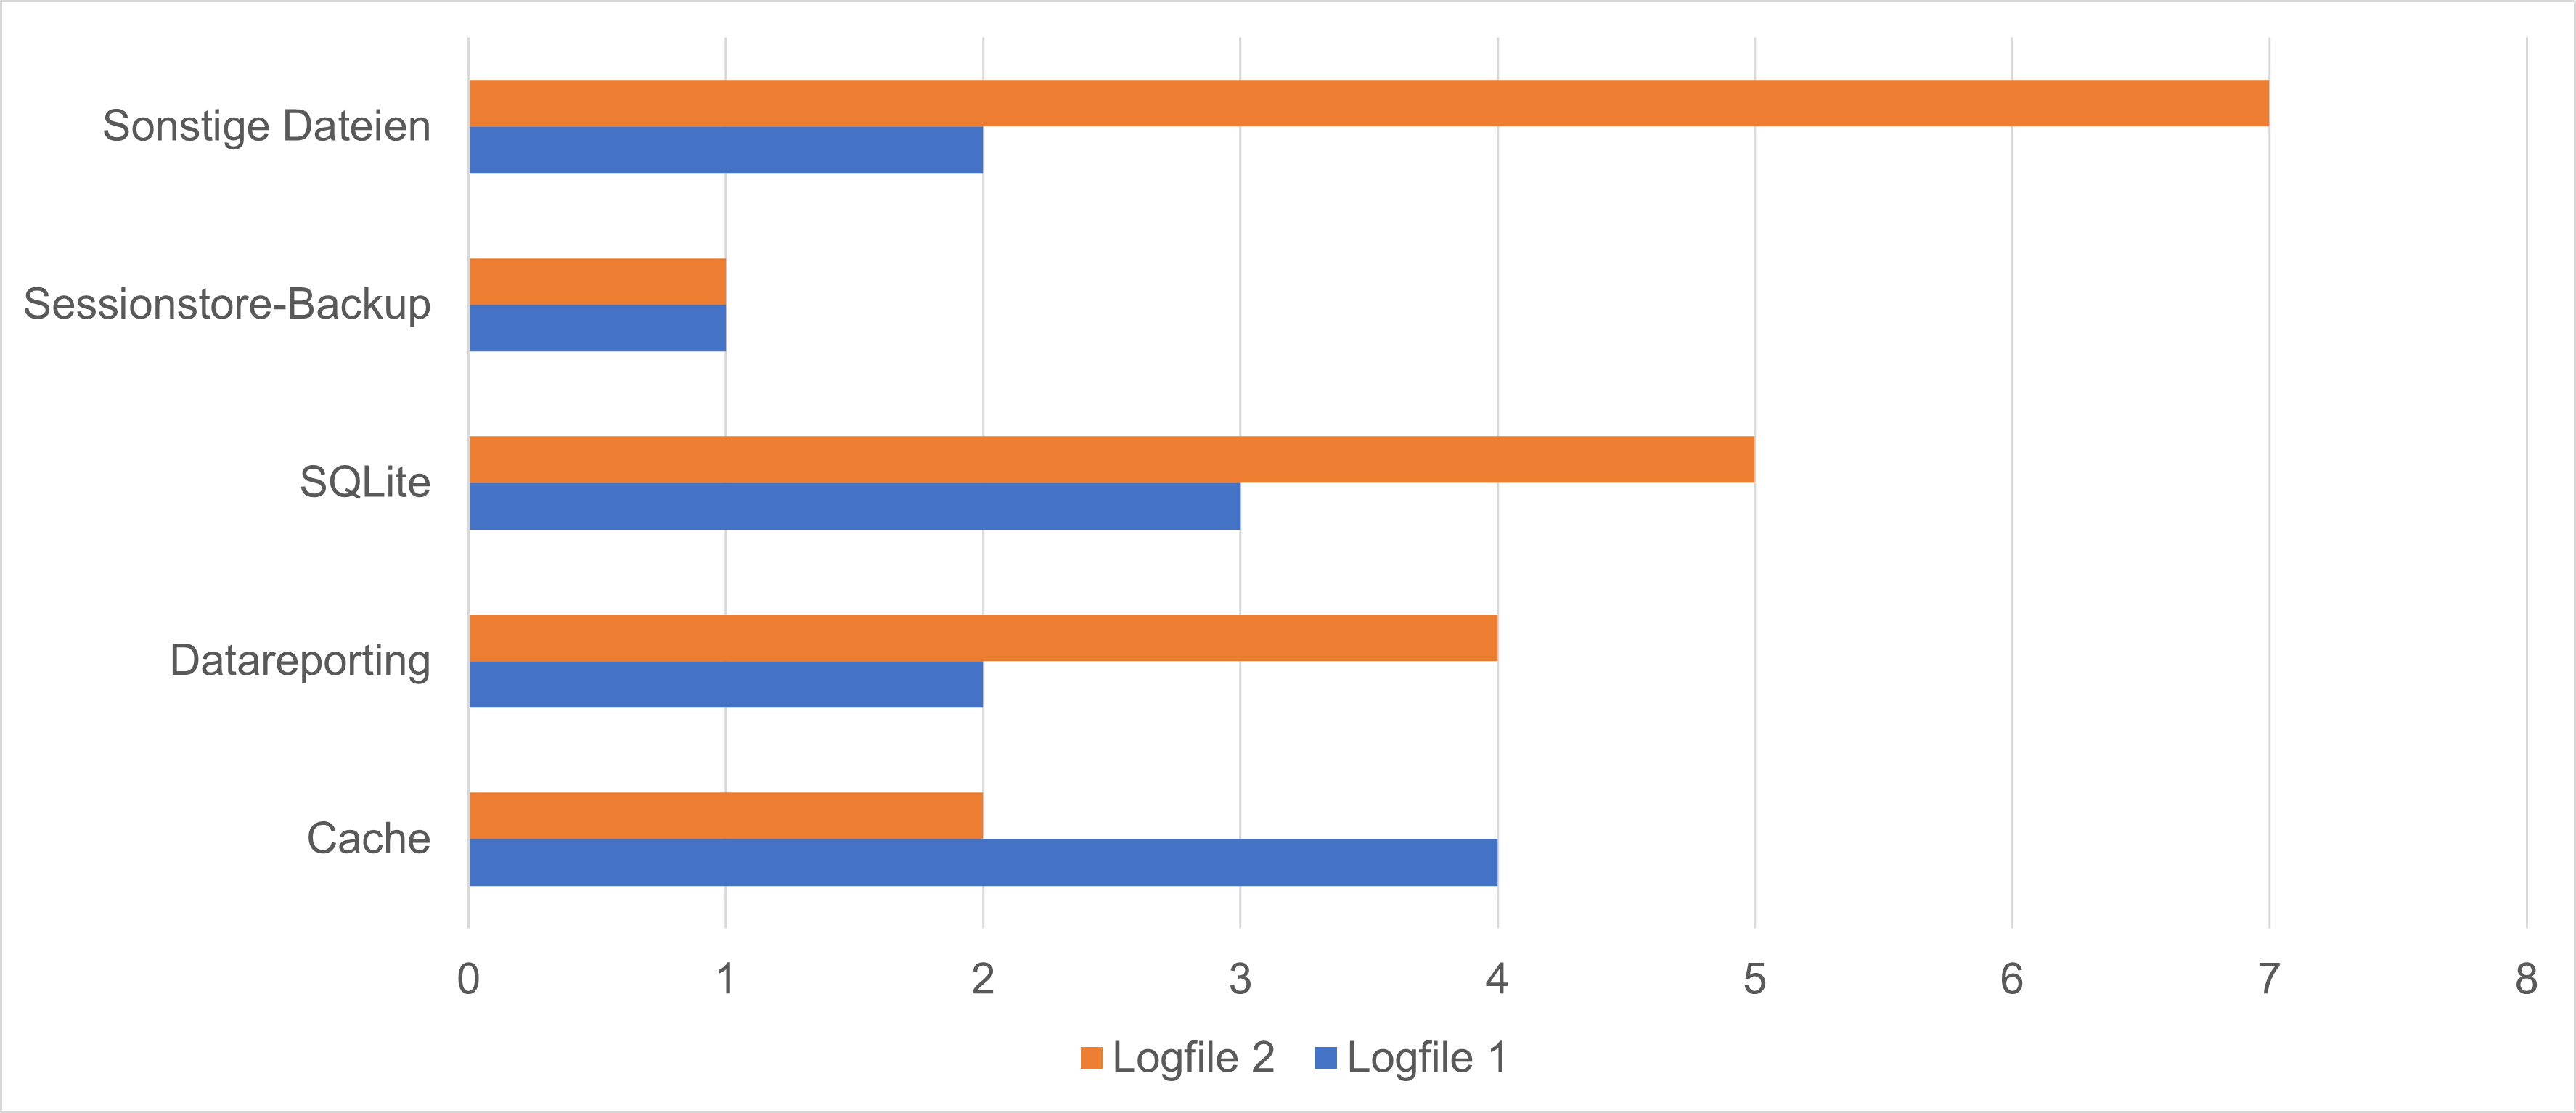
\includegraphics{bilder/bar-chart-logfile1vs2-test.png}}}
		\label{chart:final-criteria}  
		\caption{Comparison of found PB artifacts between RAM Dumps}
	\end{figure}

%Literatur:
%	o no traces were found in “common locations” \cite{Montasari.2015}
%		>  “places.sqlite”, “webappsstore. sqlite”, “sessionstore.bak”, “search.json” and “nssckbi.dll”
%	o	Safebrowsing: Alle Dateien in /safebrowsing-updating/ nicht relevant. Dort nur .vlpset und .sbstore Dateien. Speichern 256-Bit Hash von URLs, die auf SafeSearch Blacklist stehen 
%	o	Cache-Dateien: drei Caches: startupCache, jumpListCache (beide enthalten Binärdateien ohne Browsing Artefakte) und cache2 (können mit MozillaCacheView untersucht werden, enthalten keine Browsing Artefakte)
%	o	SQLite Datenbanken: Sqlite Dateien erst ohne WAL Dateien untersuchen, Danach mit sqlite3 Konsole: WAL in Datenbank schreiben mit: PRAGMA wal\_checkpoint; places.sqlite besonders relevant, da dort Browser in public Modus Browsing URLs verwaltet (Am besten hier vergleich mit Public Browsing machen)	
%		> \cite{Fayyad.2021} for Mozilla Firefox, 7 database files were recovered: cookies.sqlite-shm, places.sqlite-shm, prefs.js etc.
%		> \cite{Muir.2019} The two SQLite databases used by Firefox to track cookies and history (cookies.sqlite und places.sqlite) were both recoverable from the file system after deletion	
%		Ergebnisse stehen im Gegensatz zu \cite{Hedberg.2013} :
%			o	Chrome und Firefox: Einträge in places.sqlite + history.sqlite DB gefunden während PB! (Noch aktuell??)
%		Sonderfall: SQlite DB-Crash \cite{Hedberg.2013}
%			> WAL Files/Journal Files bei Crash gefunden -> Kann genutzt werden um zu beweisen, dass privater Browser genutzt wurde
%			> Daher: WAL Rollback mit sqlite3	
%	o	Jsonlz4 \& balkz4: Enthalten komprimierte Firefox-Sessions, jsonlz4 Dateien können mit Tool "entkomprimiert" werden: https://www.jeffersonscher.com/ffu/scrounger.html


\subsection*{Registry}
> Process Monitor: SetValue Operationen von Browser 
TODO: Logfile 1 vs 2?
	Kategorien Registry Keys:
	1) PreXULSkeletonUISettings:
		> Prefix: Absoluter Installationspfad von Firefox
		> Skeleton UI Einstellungen von Firefox % https://itigic.com/skeleton-ui-new-firefox-interface-to-start-up-much-faster/#google_vignette
			Definition:
				> Der "PreXULSkeletonUISettings" Registry Key enthielt Einstellungen für die Benutzeroberfläche (UI) des Firefox-Browsers, insbesondere für das sogenannte "Skeleton UI". Das Skeleton UI ist eine vereinfachte Benutzeroberfläche, die während des Ladens des Browsers angezeigt wird, bevor die vollständige Benutzeroberfläche geladen ist. Es besteht aus grundlegenden Steuerelementen und Elementen, die dem Benutzer die Interaktion ermöglichen, während der Rest der Benutzeroberfläche noch geladen wird.
				> Der "PreXULSkeletonUISettings"-Schlüssel enthielt Konfigurationsoptionen wie Farben, Positionen und andere Einstellungen für das Skeleton UI. Durch das Bearbeiten dieses Schlüssels konnten Benutzer die Darstellung des Skeleton UI anpassen. Es ist jedoch wichtig zu beachten, dass das Ändern der Registrierungseinträge ein fortgeschrittenes Verfahren ist und Fehler zu Problemen mit dem Browser führen kann.
			
		> Struktur der Keys: % HKCU\SOFTWARE\Mozilla\Firefox\PreXULSkeletonUISettings\C:\Program Files\Mozilla Firefox\firefox.exe|<UI Einstellung>
		> Unterschiedliche UI Einstellungen
			- % ScreenX (DWORD)
			- % ScreenY (DWORD)
			- % Width (DWORD)
			- % Height (DWORD)
			- % Maximized (DWORD)
			- % Flags (DWORD)
			- % CssToDevPixelScaling (REG_BINARY)
			- % UrlbarCSSSpan (REG_BINARY)
			- % SearchbarCSSSpan (REG_BINARY)
			- % SpringsCSSSpan (REG_BINARY)
		> keine PB Artefakte unter UI Einstellungen	
	2) Business Activity Monitoring % https://learn.microsoft.com/de-de/biztalk/core/business-activity-monitoring-bam
		> Quelle: % https://notes.qazeer.io/dfir/windows/_artefacts_overview
		> BAM is a mostly undocumented feature that controls the programs executed in the background. DAM is a feature for devices supporting the "Connected Standby" mode (i.e when a device is turned on, but its display will be turned off). As a result, the BAM registry keys will contain data on any devices, while DAM registry keys will only contain data on mobile devices.
		> The BAM registry key contains multiple subkeys under bam\\State\\UserSettings, with one subkey per user, identified with the user SID. While the key is in the SYSTEM registry hive, program executions can thus still be tied to a specific user using this SID.
		> Each user-specific key contains a list of executed programs, with their full path and timestamp of last execution.
		> If a file is deleted, the eventual associated entry in the BAM is deleted as well after the system reboot. Additionally, BAM entries older than 7 days are deleted upon system boot. The BAM thus provides limited information on historic execution of programs
		> No entries are created in the BAM keys for executables on removable media and/or on network shares.
		> Key: %  HKLM\System\CurrentControlSet\Services\bam\State\UserSettings\S-1-5-21-588412547-2749917301-3803556669-1001\\Device\HarddiskVolume2\Program Files\Mozilla Firefox\firefox.exe (REG_BINARY)

Quantitativ: (Diagramme)
	- Stacked Balkendiagramm jeweils für Logfile 1 und Logfile2: Anteil Kategorie 1 bzw.2 an allen Registry-Schreiboperationen
	\begin{figure}[h!]
		\centerline{\resizebox{\linewidth}{!}{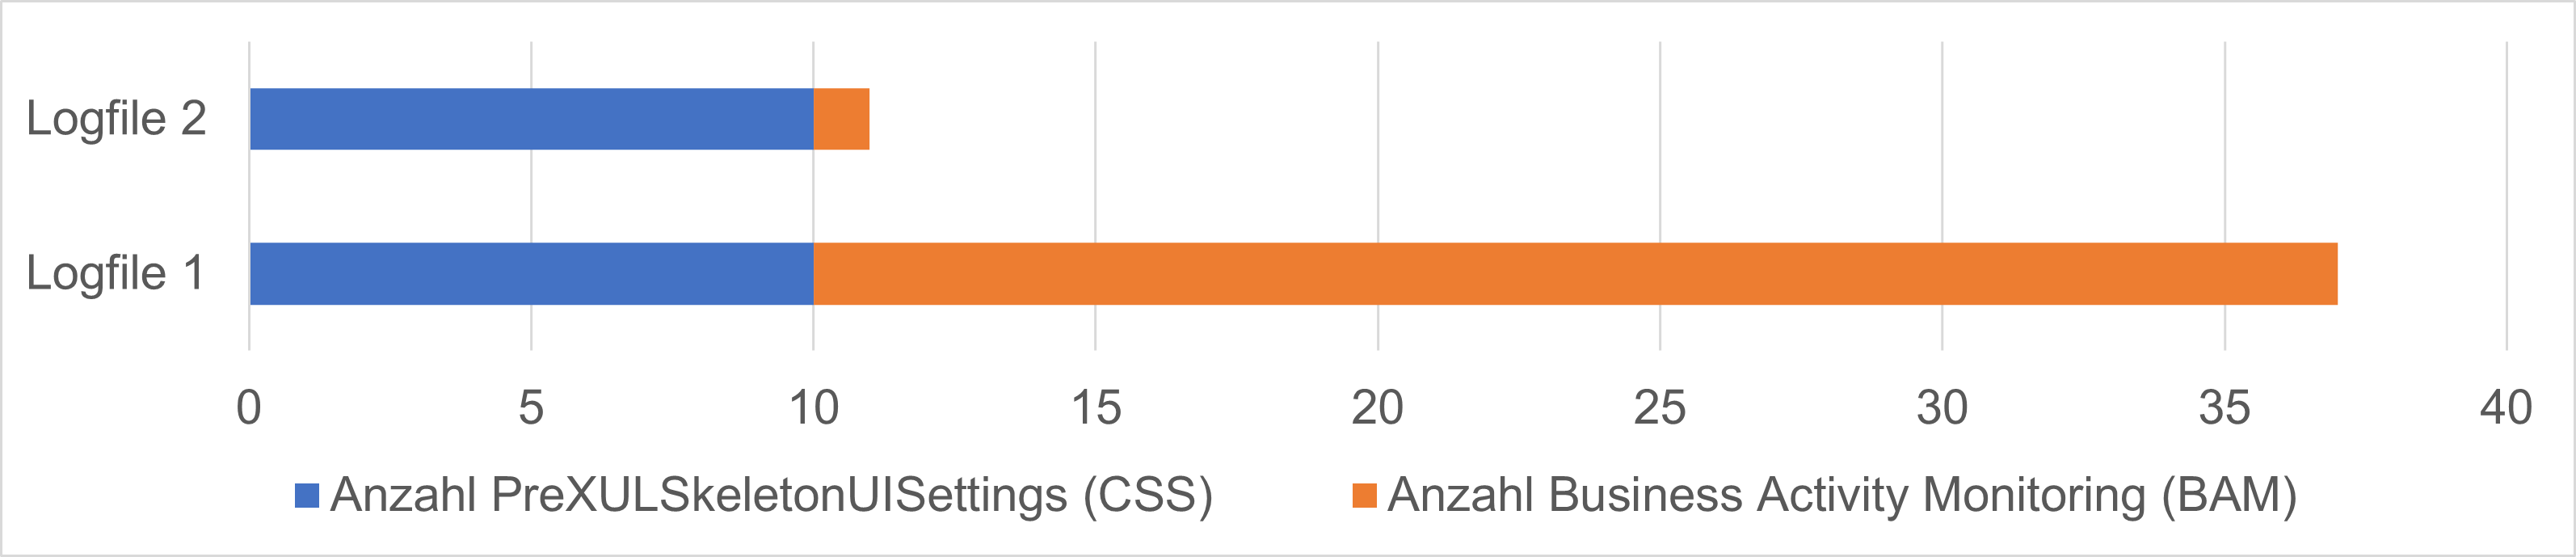
\includegraphics{bilder/firefox-registry-stacked-bar-chart.png}}}
		\label{chart:final-criteria}  
		\caption{Comparison of found PB artifacts between RAM Dumps}
	\end{figure}
	
> Stringsuche in Registry Hives mit Registry Explorer (Siehe Liste)
	In allen Hives kein Treffer für alle Suchbegriffe

Literatur: 
	> angeblich in Shellactivities Ergebnisse. --> Nicht mehr vorhanden in aktueller Version (Verweis auf E-Mail)

%Literatur:
%	>	Auf Autor verweisen: angeblich in Shellactivities Ergebnisse. --> Nicht mehr vorhanden in aktueller Version (Verweis auf E-Mail)
%	>	Process Monitor/Regshot zeigen keine relevanten Key-Änderungen
%	> \cite{Muir.2019}: Autopsy Keyword Suche nach Suchbegriffen: Ergebnisse in \%SystemRoot\%Minidump NTUSER.DAT, ntuser.dat.LOG1 (a log of changes to NTUSER.DAT)
%	> Zentral: shellactivites Key:	NTUSER.DAT --> “shellactivities” key \cite{Muir.2019}
%	> \cite{Rochmadi.2017} Detection of registry changes helps to determine what the appropriate plugin is used to search for digital evidence using volatility memory forensic:
%	- RegQueryValue:	HKCU/Software/Microsoft/Windows/CurrentVersion/InternetSettings/Connections/DefaultConnectionSettings
%	- RegCloseValue: 	HKCU/Software/Microsoft/Windows/CurrentVersion/InternetSettings/Connections
%	- IRP\_MJ\_READ: C:/pagefile.sys

\subsection*{Black-Box Analyse/Uncommon Locations}

\subsubsection*{Analyse mit Autopsy}
Bei White-Box Analyse/Common Locations: Autopsy nur zur Dateiextraktion genutzt, hier: als konkretes forensisches Werkzeug

Stichwortsuche:
- In allen Snapshots keine Treffer (auch innerhalb \$Carved)
- TODO: Pagefile gefunden?

Von Autopsy automatisch indexierte Dateien: 
In allen Fällen: keine Dateien gelöscht, nur über Zeitraum der Snapshots neue dazugekommen
- Web Bookmarks:
	\begin{figure}[h!]
		\centerline{\resizebox{\linewidth}{!}{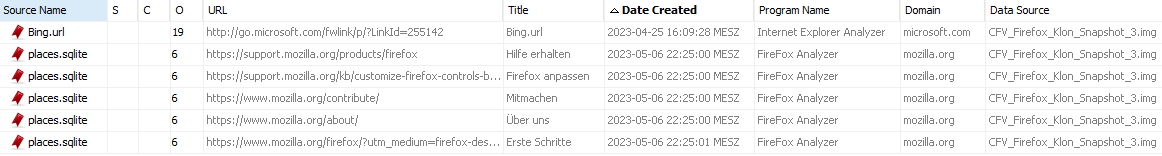
\includegraphics{bilder/cfv_firefox_autopsy_web_bookmarks.png}}}
		\label{chart:final-criteria}  
		\caption{Autopsy Web Bookmarks}
	\end{figure}
	Snapshot 1:
		> Bing.url (Unter C:/User/Forensik/Favorites/Links) enthält Bing Startseite
	Snapshot 2:
		> 5 Einträge in places.sqlite: (Firefox Standardseiten -> Deckt sich mit Beobachtungen aus Process Monitor Analyse, siehe Kapitel X)
	Snapshot 3:
		> unverändert zu 2
	Snapshot 4:
		> unverändert zu 3
- Web Cookies:
	\begin{figure}[h!]
		\centerline{\resizebox{\linewidth}{!}{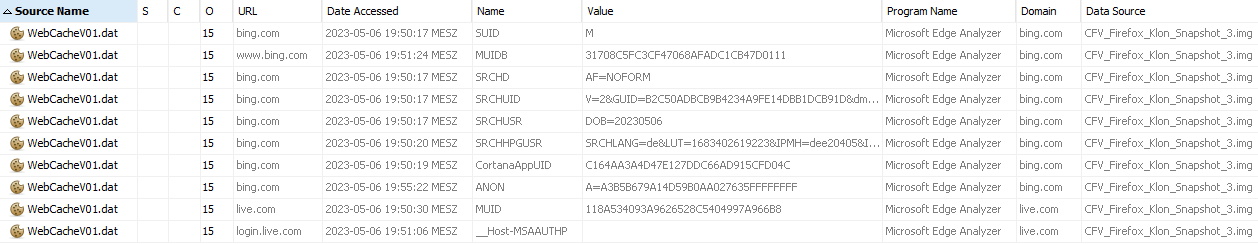
\includegraphics{bilder/cfv_firefox_autopsy_web_cookies.png}}}
		\label{chart:final-criteria}  
		\caption{Autopsy Web Cookies}
	\end{figure}
	Snapshot 1:
		> 10 Einträge in WebCacheV01.dat (= DB des Internet Explorers zum speichern von Browserdaten): Cookies für bing.com und live.com (= outlook)
	Snapshot 2:
		> unverändert zu 1
	Snapshot 3:
		> unverändert zu 2
	Snapshot 4:
		> unverändert zu 3
- Web History:
	\begin{figure}[h!]
		\centerline{\resizebox{\linewidth}{!}{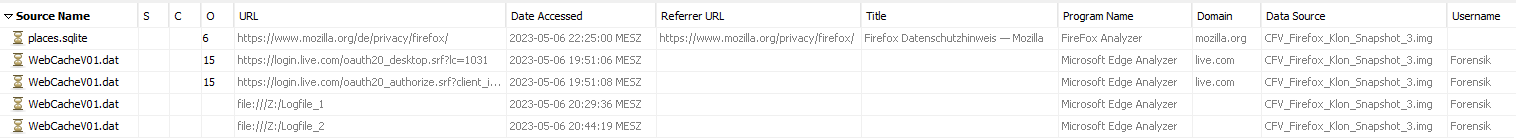
\includegraphics{bilder/cfv_firefox_autopsy_web_history.png}}}
		\label{chart:final-criteria}  
		\caption{Autopsy Web History}
	\end{figure}
	Snapshot 1:
		> 2 Einträge in WebCacheV01.dat:
			- 2x live.com (= outlook)
	Snapshot 2:
		> 1 Eintrag in places.sqlite: % https://www.mozilla.org/privacy/firefox/
			-> Zurückzuführen auf Seite, die sich automatisch geöffnet hat, als Firefox gestartet (bevor privates Fenster geöffnet wurde)
		> 1 neuer Einträge in WebCacheV01.dat:
			- file:///Z:/Logfile\_1 (= Process Monitor Logfile, die in shared-Folder geladen wurde) -> Erklärung?
	Snapshot 3:
		> 1 neuer Eintrag in WebCacheV01.dat:
			- file:///Z:/Logfile\_2 (= Process Monitor Logfile, die in shared-Folder geladen wurde) -> Erklärung?
	Snapshot 4:
		> unverändert zu 3
- Web Categories:
	\begin{figure}[h!]
		\centerline{\resizebox{\linewidth}{!}{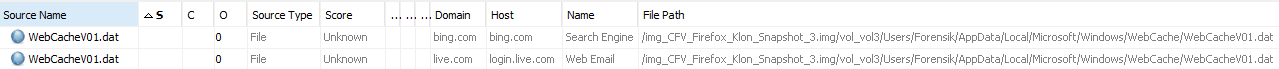
\includegraphics{bilder/cfv_firefox_autopsy_web_categories.png}}}
		\label{chart:final-criteria}  
		\caption{Autopsy Web Categories}
	\end{figure}
	Snapshot 1:
		> 2x WebCacheV01.dat aufgelistet => Mit HxD untersucht, keine PB Artefakte
	Snapshot 2:
		> unverändert zu 2
	Snapshot 3:
		> unverändert zu 3
	Snapshot 4:
		> unverändert zu 4
		
Zusammenfassung:
- keine PB Artefakte
- Keine neuen Erkenntnisse vgl. mit intensiver Analyse mittels Process Monitor in Kapitel X
- Eintrag von Datenschutzseite in places.sqlite wurde erkannt.

%Literatur:
%	o	Autopsy Keywortsuche: 
%		>	In alles Snapshots ergebnislos (keine Keyword-Hits
%		-->	In Literatur: Autoren fanden Ergebnisse in pagefile.sys 
%			> Autopsy: websites and some of the keywords found in hidden file called “pagefile.sys” \cite{Mahlous.2020}
%			o \cite{Montasari.2015} traces were found in: 
%				> However, on investigating the “pagefile.sys”, some entries were discovered
%				> Using the “data carving” technique, profile picture was recovered
%			o \cite{Said.2011} 
%				> Examining pagefile.sys showed some positive hits 			
%		--> Evtl. hier zeigen, was gefunden werden kann, wenn RAM reduziert
%		--> Aber auf Problem hinweisen, dass gefundener String in pagefile nicht direkt Browser zugeordnet werden kann
%		> \cite{Gabet.2018}	Firefox only produced three recoverable artefacts as reported by both tools (FTK, Autopsy) --> Artefakte werden nicht genannt!
%		> \cite{Muir.2019} Autopsy Keyword Suche nach Suchbegriffen: unallocated space
%		> Autopsy Carving Module (\$Carved): \cite{Muir.2019}
%			•	When searching for the string ’clot’ from the browsing protocol, six .dll, .edb and .reg files were discovered in unallocated space.
%			•	Further searching of unallocated space uncovered references to the Tor installation directory and the obfs4 bridging IP addresses
%			•	browsing data found in NTUSER.DAT was also replicated in unallocated space.
%	o	Autopsy PlugIns:
%		>	*** TODO: Hier Liste mit PlugIns ***

\subsubsection*{Analyse mit Volatility}
Vorgehen: Siehe "Methodik" Kapitel
	- Ausgangslage: Volatility Yarascan Treffer
	- Für jeden Treffer: virtueller Offset des Strings, PID, getriggerte Yararule, getriggerte Yara Component z(= Variablenname des gesuchten Strings), gefundener String
	- Neue Spalte: "Prozessname" -> zu jeder PID Prozessnamen
	- Ergebnisse Aufbereitet nach folgendem Schema:
		> Für jeden RAM Dump
		> Für jede Yararule
		> Für jede Component
		> Filter: Prozessname = Firefox -> Anzahl zählen
		> Filter: Prozessname = Alle Prozesse außer Firefox -> Anzahl zählen

Yararule "Keyword":
	\begin{figure}[h!]
		\centerline{\resizebox{\linewidth}{!}{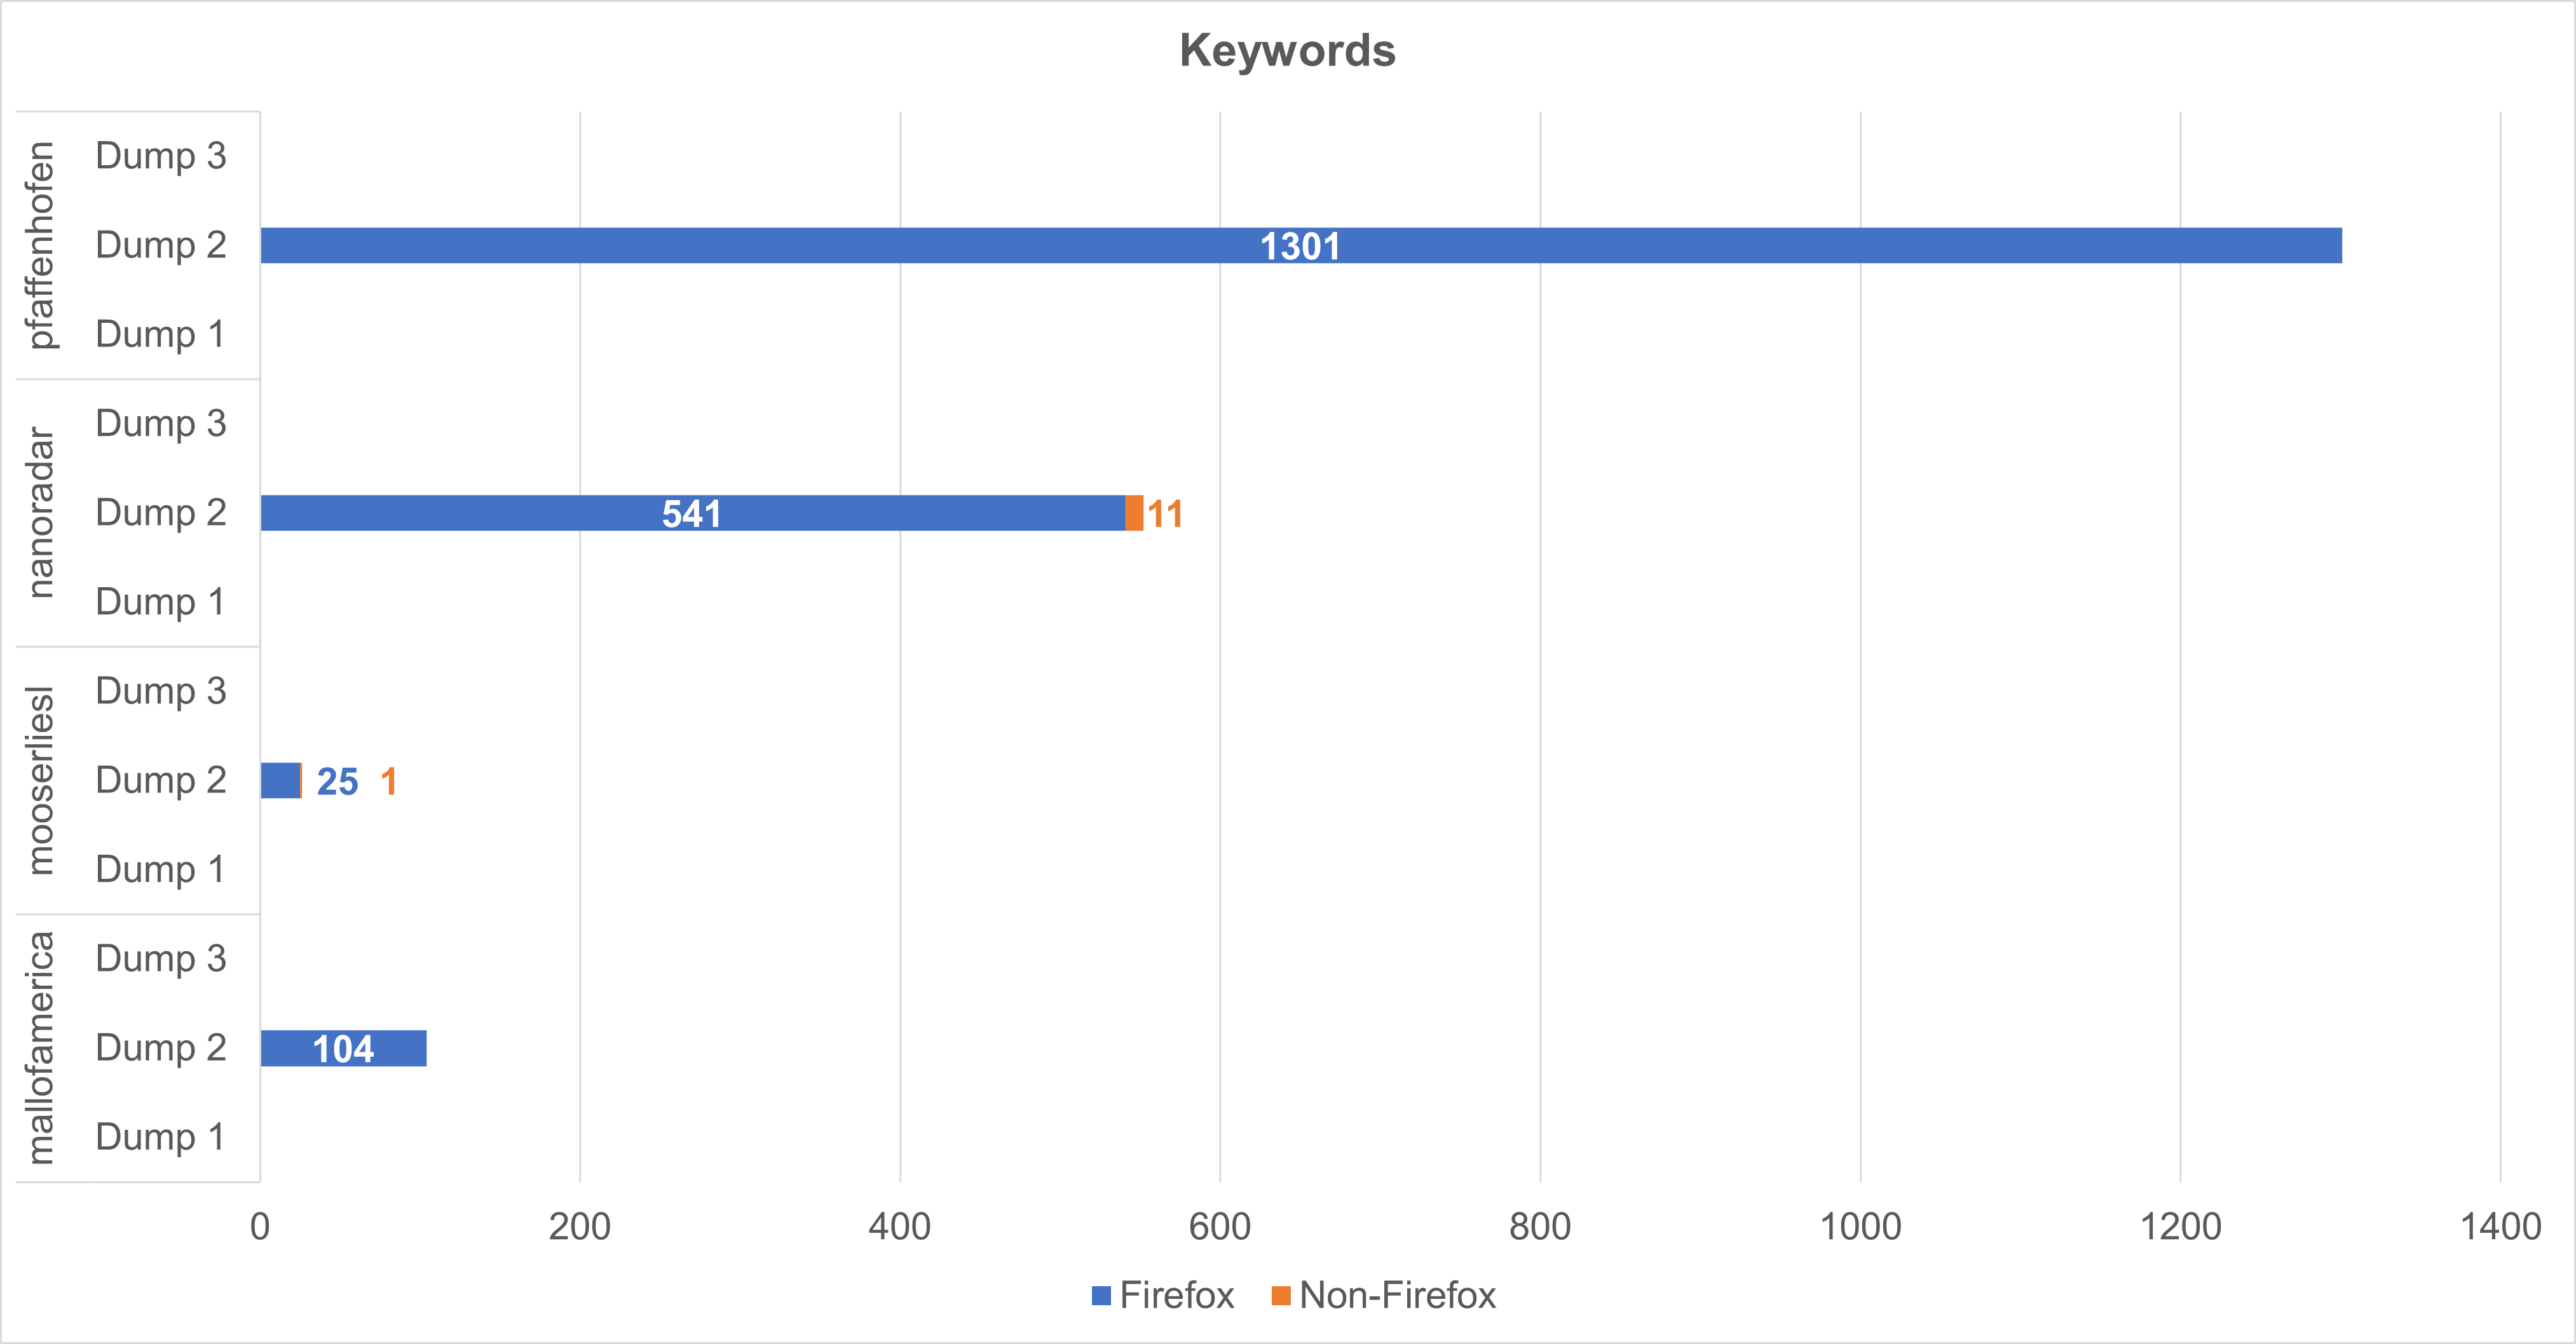
\includegraphics{bilder/volatility/firefox/keywords.png}}}
		\label{chart:final-criteria}  
		\caption{Keywords}
	\end{figure}
	Analyse:
		> Ausschließlich in RAM Dump 2 Keyword Artefakte gefunden
		> Hauptsächlich in Firefox Prozess
		> Mit 1301 Artefakten, am häufigsten pfaffenhofen vertreten. Vermutung: Evtl. weil Google Maps viele zusätzliche Artefakte lädt. 
		
Yararule "URL":
	\begin{figure}[h!]
		\centerline{\resizebox{\linewidth}{!}{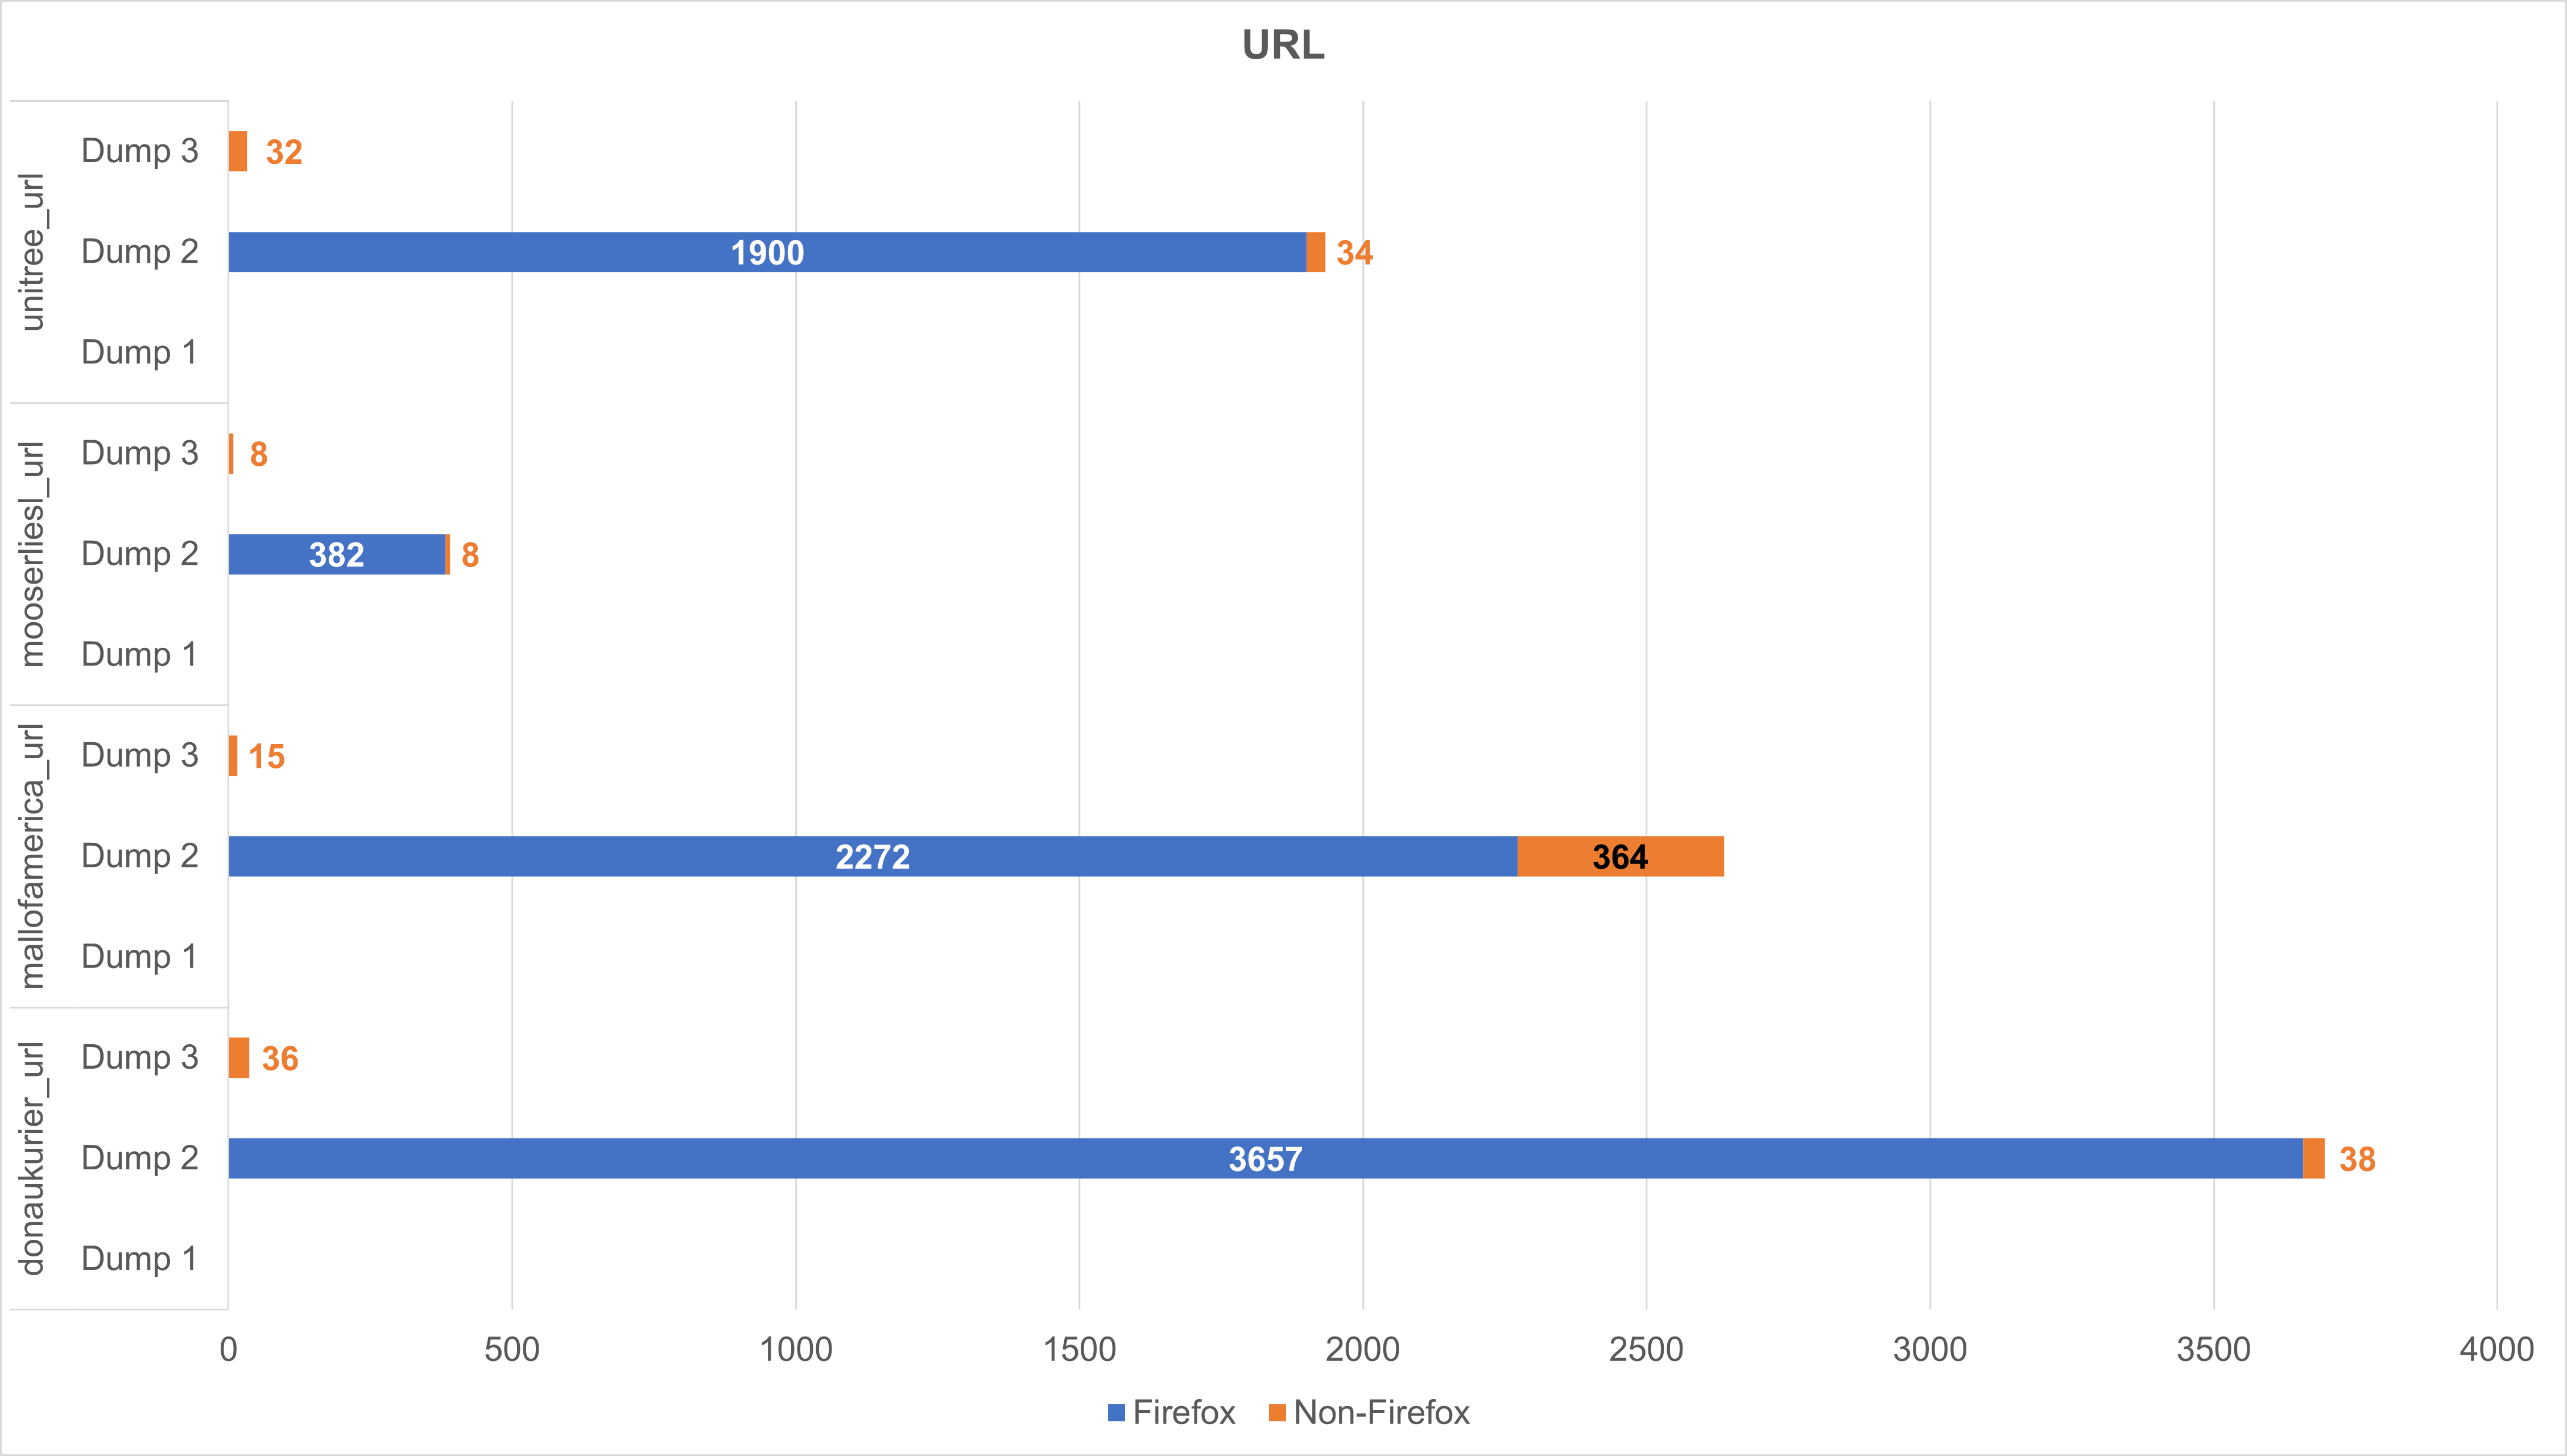
\includegraphics{bilder/volatility/firefox/url.png}}}
		\label{chart:final-criteria}  
		\caption{URL}
	\end{figure}
	Analyse:
		> Wie bei anderen Kategorien: Die meisten Artefakte in RAM Dump 2, in Firefox Prozessen
		> mooserliesl tritt am wenigsten auf, donaukurier am meisten (vmtl. auf Öffnen von Bild zurückzuführen)
		> Hier bemerkenswert, dass in RAM Dump 3 Artefakte von allen vier URLs zu finden sind
		> Bei genauerer Analyse des Process Monitor Logfiles herausgefunden: Artefakte alle in svchost.exe Prozess gefunden
		> Deshalb RAM Dump erneut mit Volatility windows.svcscan Plugin untersucht:
			"The svcscan plugin allows the analyst to list out the services running. This plugin gives more detail to the running processes in the event that the analyst requires additional details such as the display name, binary path, or service type." % (https://www.oreilly.com/library/view/digital-forensics-and/9781787288683/9ab60586-2b04-45e0-b437-dbfe10ab3be8.xhtml)
		> Ausgabe aller im RAM gefundener Services
		> Problem: Volatility svcscan liefert keine PID zu laufenden Services
		> Deshalb: "White-Box" Analyse: Snapshot 3 erneut aufgetaut, danach mit Process Explorer PID X (TODO!) von SVChost Prozess gesucht, in dem PB Artefakte gefunden wurden
			Def. Process Explorer:
				"Prozess Explorer zeigt Ihnen Informationen darüber an, welche Handles und DLLs-Prozesse geöffnet oder geladen wurden." % https://learn.microsoft.com/de-de/sysinternals/downloads/process-explorer
				"Process Explorer, from Sysinternals, is a process management program that allows you to see the running processes on your computer and a great deal of information about each process. One of the nice features of Process Explorer is that it also gives you the ability to see what services a particular SVCHOST.EXE process is controlling."
		> Ergebnis: DNSCache Service mit PID X (TODO!) = DNScache Service
			TODO: Screenshot
		> Ausführung von ipconfig /displaydns liefert gecachte URLs
			TODO: Screenshot
		> Nach Löschen des DNSCaches mit ipconfig /flushdns + Schließen aller Process Monitor Instanzen + Beenden des DNSCaches Services + Erneuter RAM-Dump -> Keine PB Artefakte mehr gefunden!
Yararule "Mail":
	\begin{figure}[h!]
		\centerline{\resizebox{\linewidth}{!}{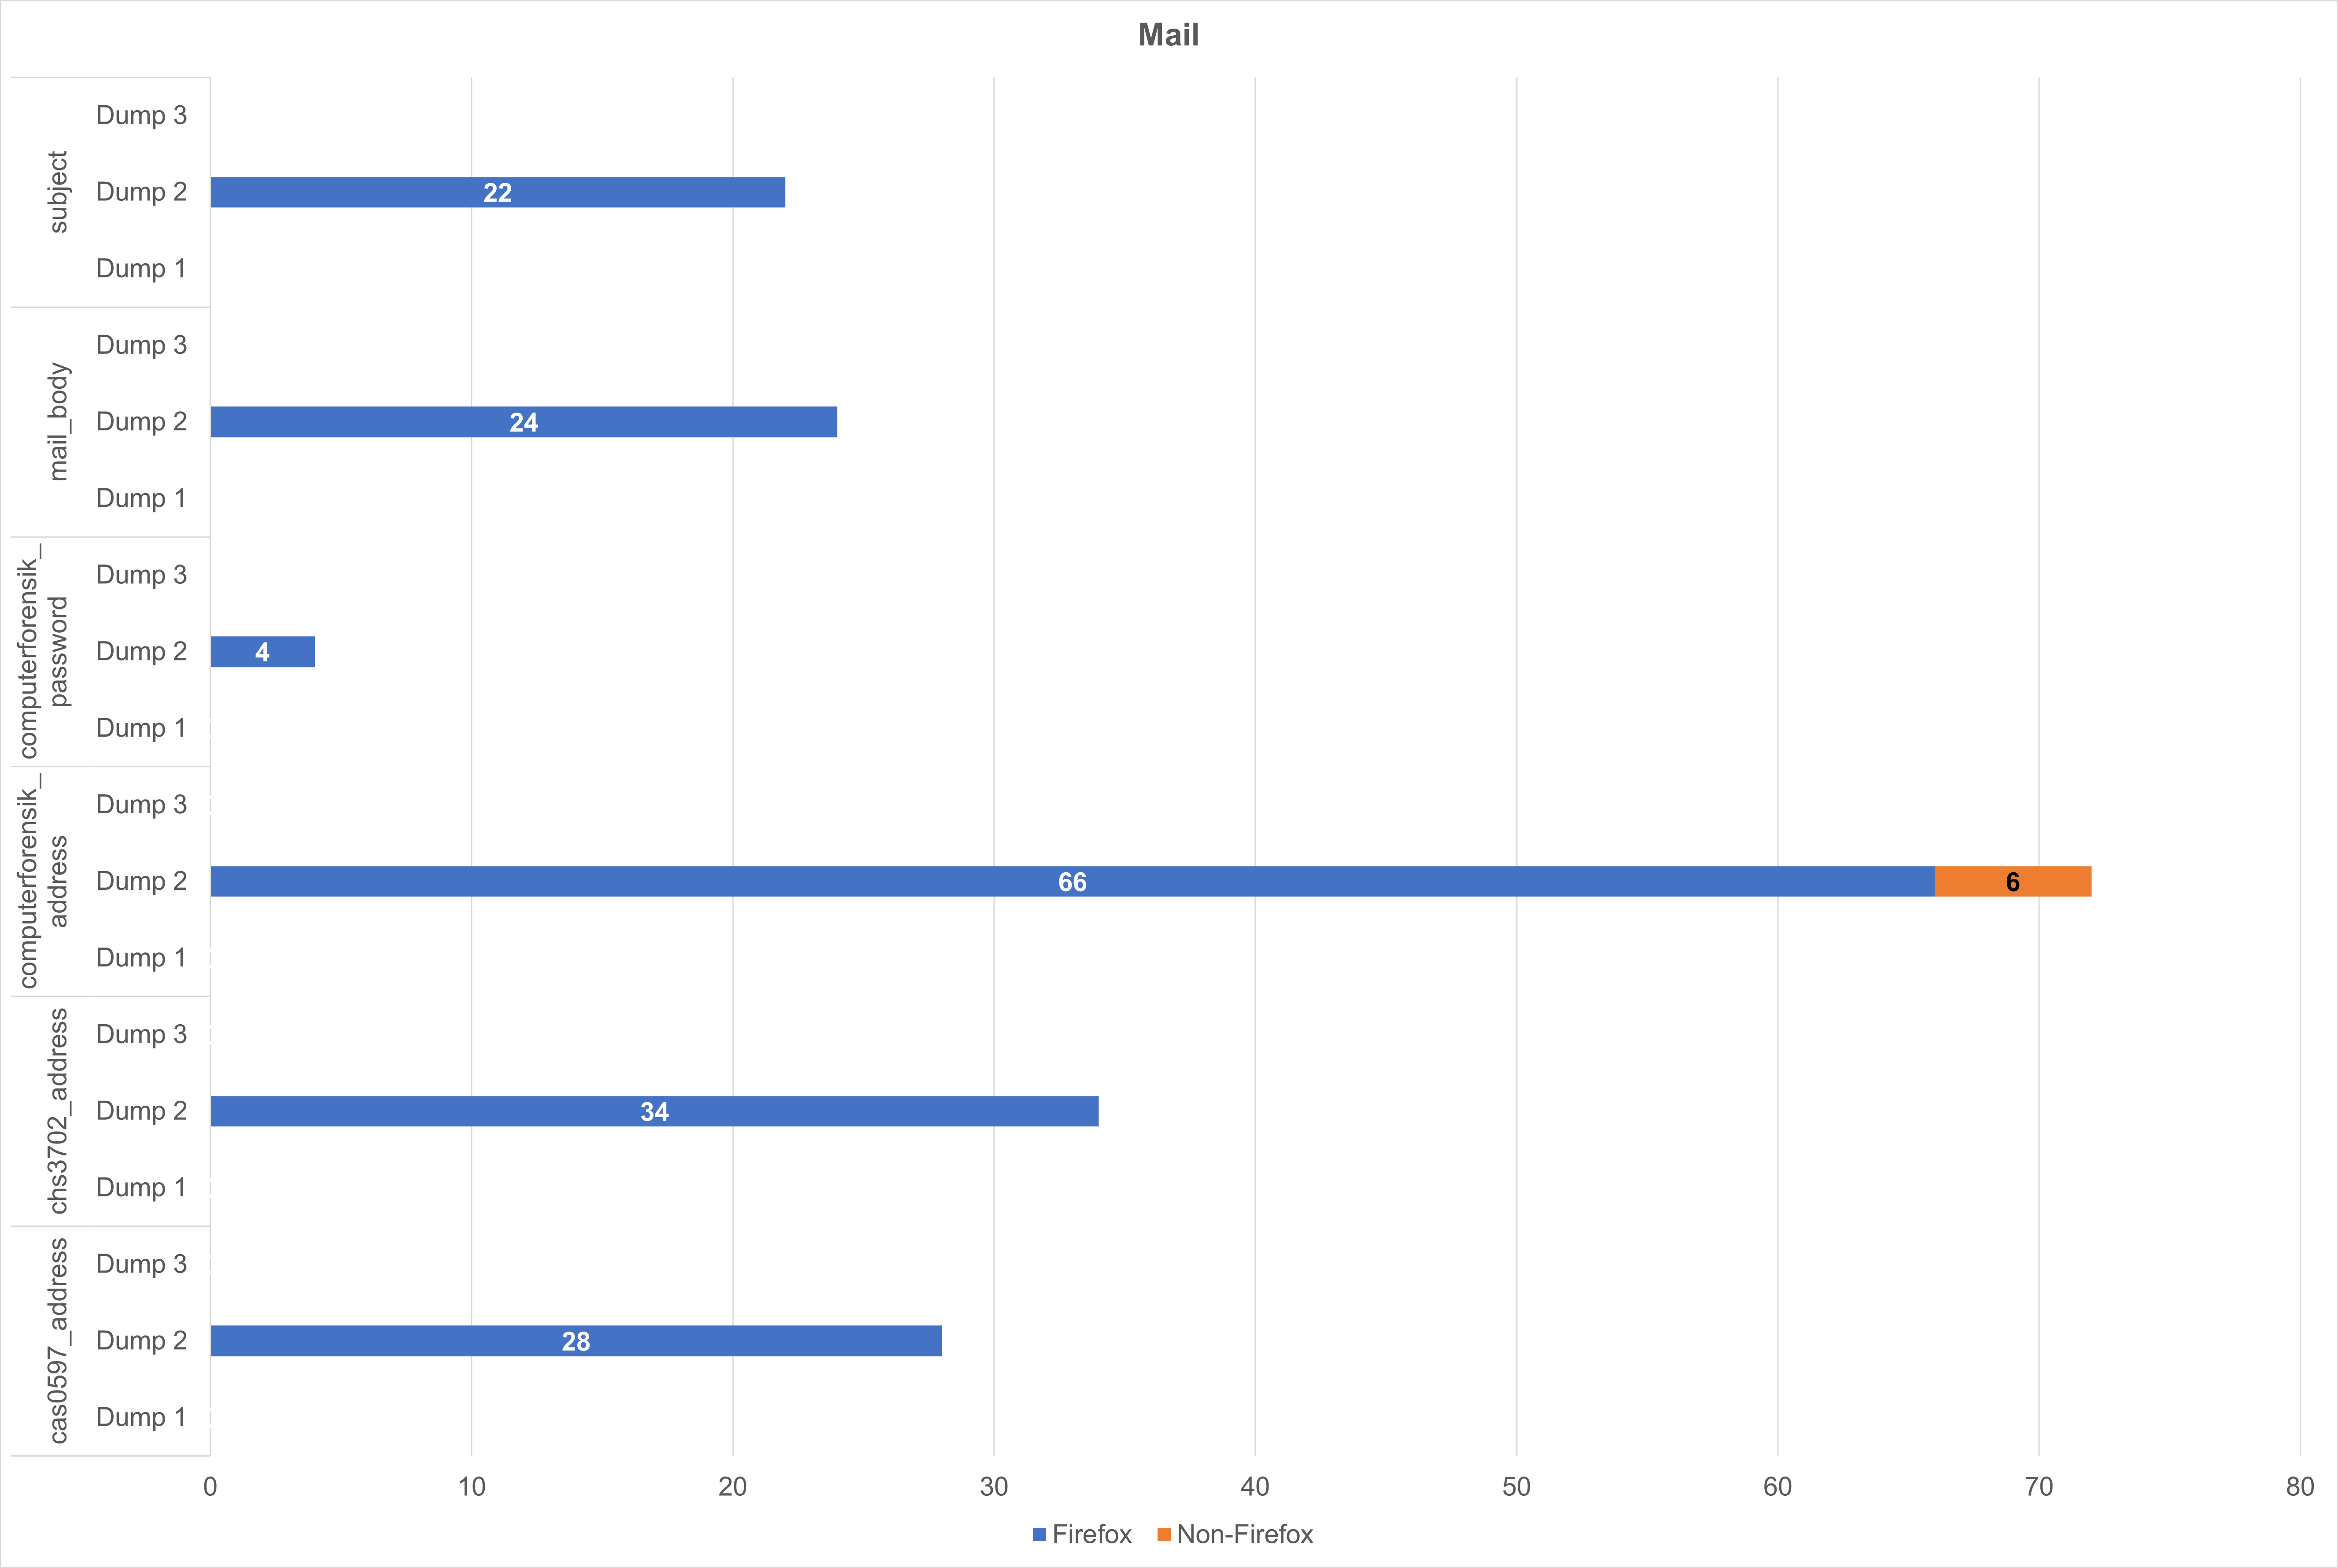
\includegraphics{bilder/volatility/firefox/mail.png}}}
		\label{chart:final-criteria}  
		\caption{Mail}
	\end{figure}
	Analyse:
		> Alle Mail Artefakte gefunden
		> Ausschließlich in RAM Dump 2 Mail Artefakte gefunden
		> Am häufigsten Absenderadresse "computerforensikvl@gmail.com" gefunden, als einziges Artefakt auch in anderen Prozessen gefunden.
		> Bemerkenswert: Passwort wurde 4x als Klartext im RAM gefunden!
			String Kontext:
				Offsets:		PIDs:
				0xb9ce29180c8	7420
				0x2859f4ffd4e0	7420
				0x24083b41858	8424
				0x240840e5b08	8424
				
			Memmap: Pid 7420
				virtual			physical	size	offset in file
				0xb9ce2918000	0xcb20a000	0x1000	0x11dd4000
					-> 0xb9ce29180c8 = 0x11dd40c8 
					\begin{figure}[h!]
						\centerline{\resizebox{0.7\linewidth}{!}{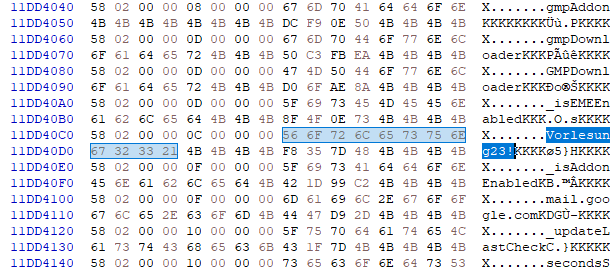
\includegraphics{bilder/volatility/firefox/password_0xb9ce29180c8_7420.png}}}
						\label{chart:final-criteria}  
						\caption{Password in memory page of PID 7420 at offset 0xb9ce29180c8}
					\end{figure}
				0x2859f4ffd000	0x96812000	0x1000	0x12e23000	Disabled				
					-> 0x2859f4ffd4e0 = 0x12e234e0
					\begin{figure}[h!]
						\centerline{\resizebox{0.7\linewidth}{!}{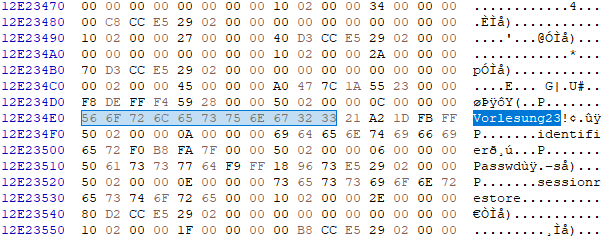
\includegraphics{bilder/volatility/firefox/password_0x2859f4ffd4e0_7420.png}}}
						\label{chart:final-criteria}  
						\caption{Password in memory page of PID 7420 at offset 0x2859f4ffd4e0}
					\end{figure}
			Memmap: Pid 8424
				virtual			physical	size	offset in file
				0x24083b41000	0xc1d52000	0x1000	0x583000	Disabled
					-> 0x24083b41858 = 0x583858
					\begin{figure}[h!]
						\centerline{\resizebox{0.7\linewidth}{!}{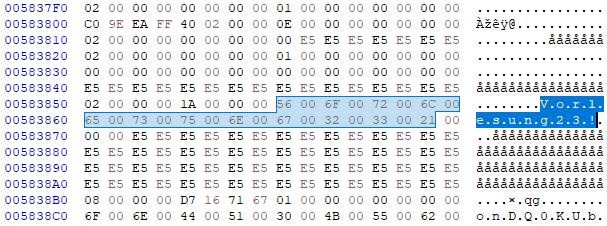
\includegraphics{bilder/volatility/firefox/password_0x24083b41858_8424.png}}}
						\label{chart:final-criteria}  
						\caption{Password in memory page of PID 8424 at offset 0x24083b41858}
					\end{figure}
				0x240840e5000	0x2d3fb000	0x1000	0x96b000	Disabled
					-> 0x240840e5b08 = 0x96bb08
					\begin{figure}[h!]
						\centerline{\resizebox{0.7\linewidth}{!}{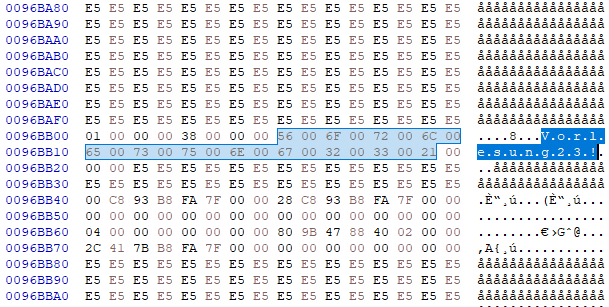
\includegraphics{bilder/volatility/firefox/password_0x240840e5b08_8424.png}}}
						\label{chart:final-criteria}  
						\caption{Password in memory page of PID 8424 at offset 0x240840e5b08}
					\end{figure}
		> In PID 8424: 2 Bytes pro Character, bspw. Unicode
				
Yararule "Image":
	\begin{figure}[h!]
		\centerline{\resizebox{\linewidth}{!}{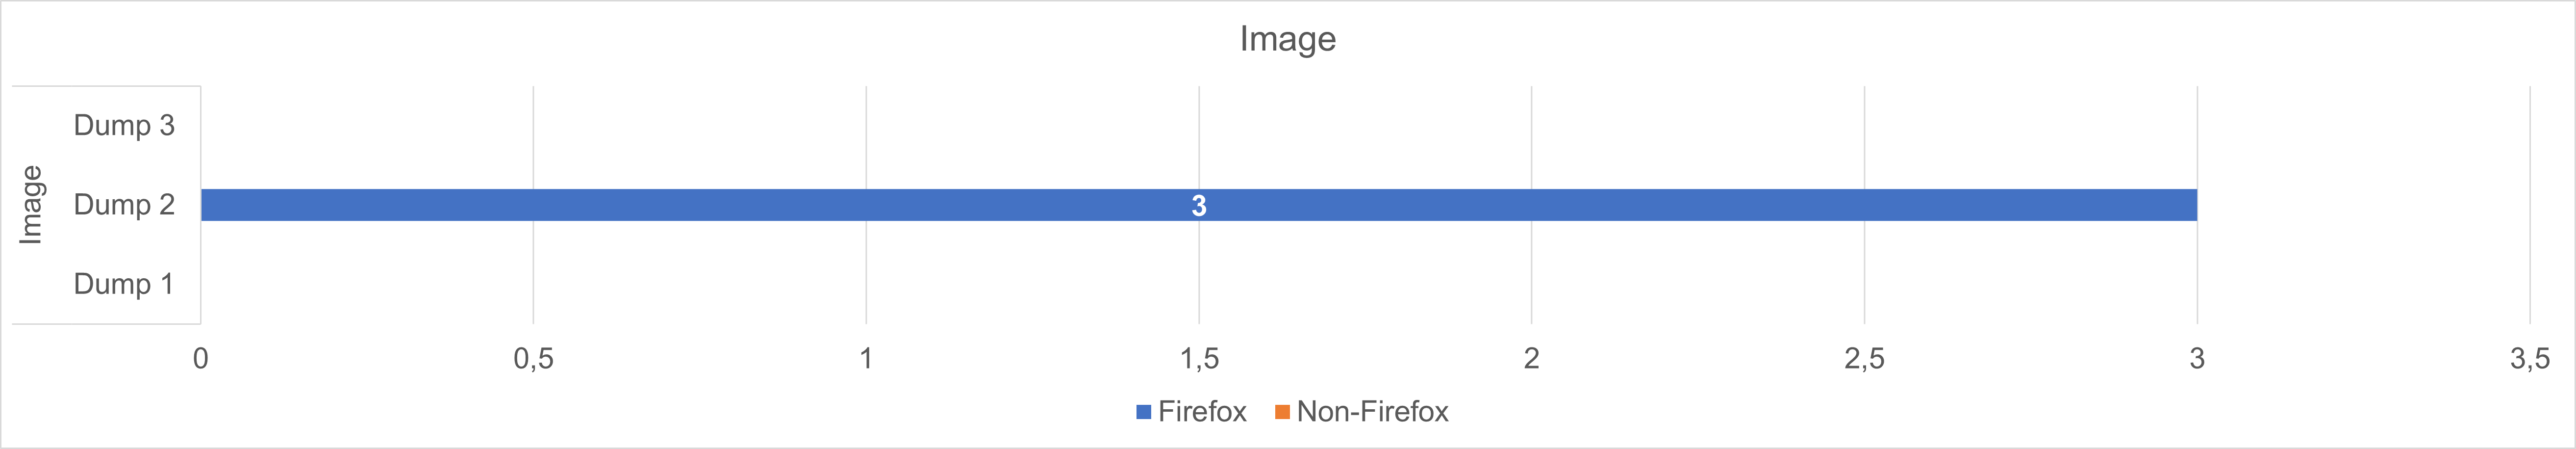
\includegraphics{bilder/volatility/firefox/image.png}}}
		\label{chart:final-criteria}  
		\caption{Image}
	\end{figure}
	Analyse:
		> Hex-Wert von Donaukurier Bild wurde im 2. RAM Dump in 3 Firefox Prozessen gefunden
	

Zusammenfassung = Stacked Bar Chart:
\begin{figure}[h!]
	\centerline{\resizebox{\linewidth}{!}{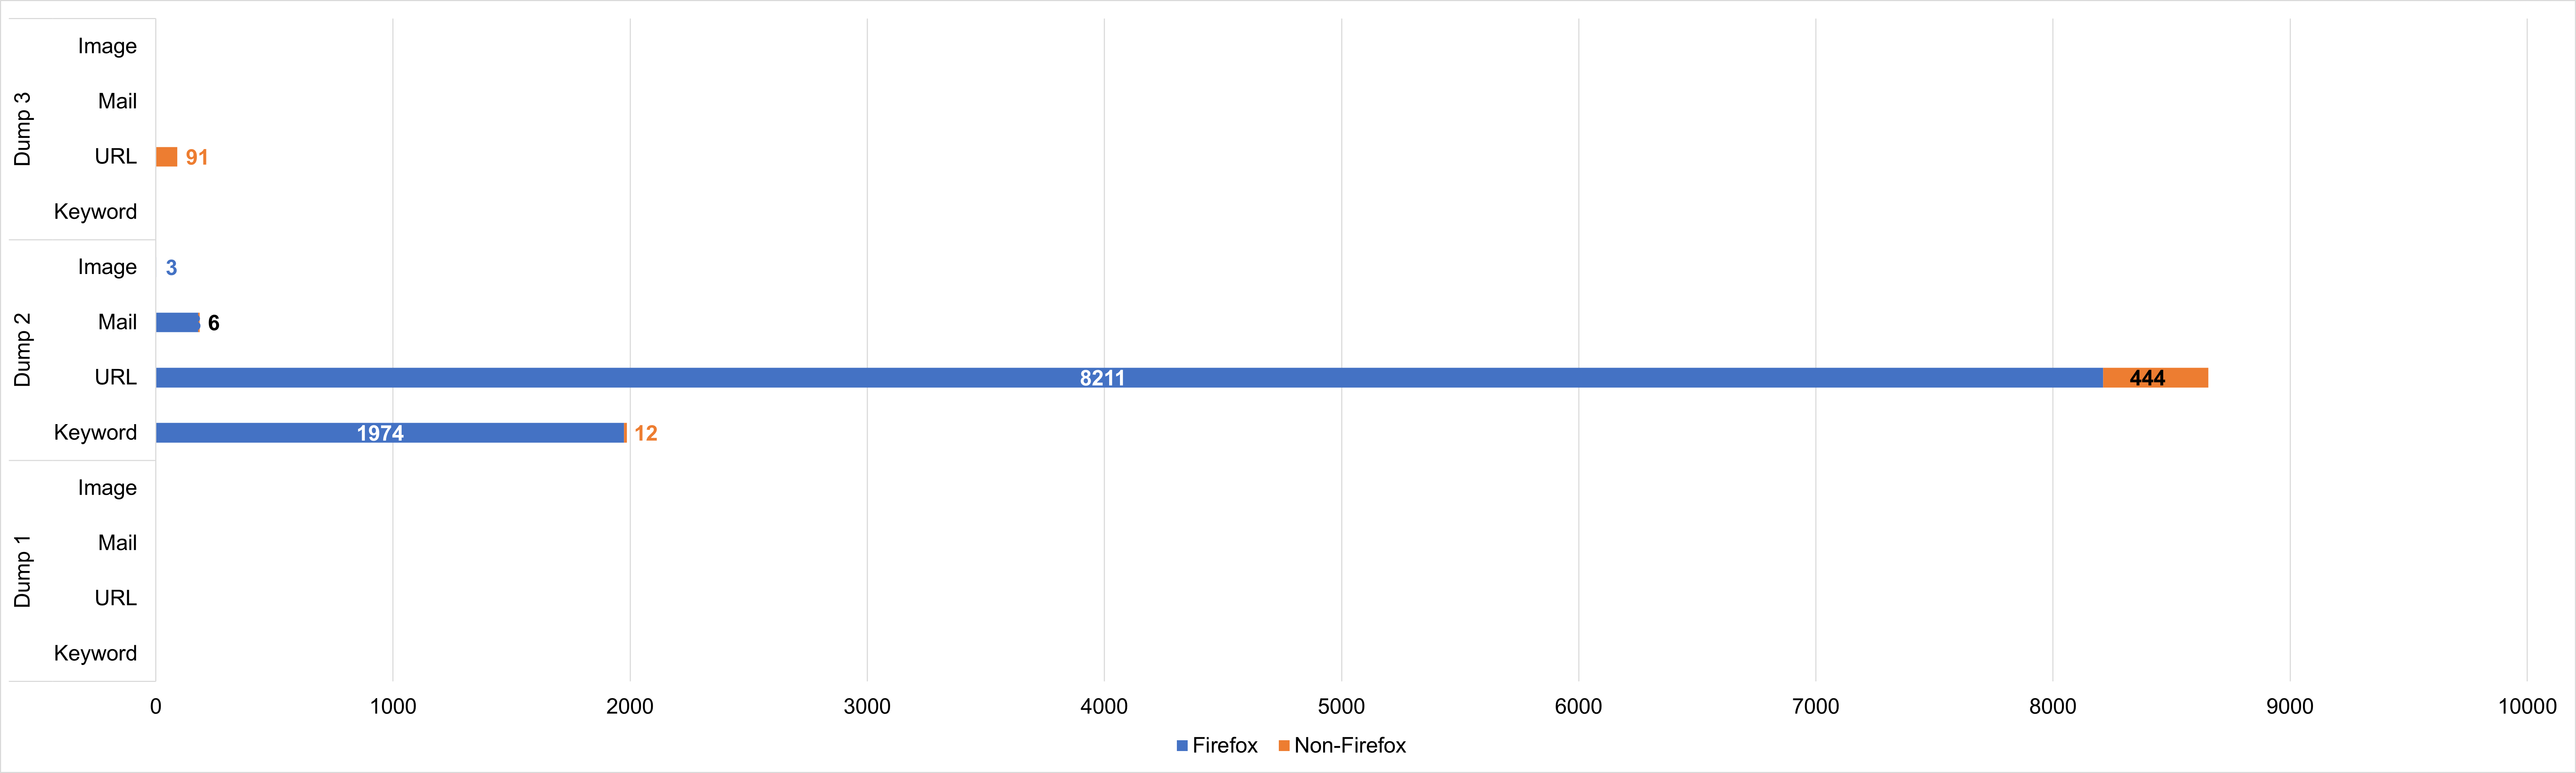
\includegraphics{bilder/volatility/firefox/summary.png}}}
	\label{chart:final-criteria}  
	\caption{Summary}
\end{figure}

TODO: Kreisdiagramme/Balkendiagramme mit Gesamtzahl an (Non-)Firefox Yarascan-Treffer erst im Vergleich mit Tor

\newpage

\section{Tor}

\subsection*{White-Box Analyse/Common Locations}

Schreiboperationen mit Process Monitor verfolgen:

Im Anhang: Tabelle mit allen geschriebenen Dateien (markiert, wenn nicht mehr wiederherstellbar + markiert, wenn Datei "verändert" (siehe oben: temp, WAL))

Aux-Dateien, welche nicht mehr vorhanden waren, aber dafür "richtige" Dateien:
	- % *\datareporting\glean\db\data.safe
	- % *\datareporting\archived\2023-05\1683405837882.9102466b-e465-4ecb-810f-74ae90c64c63.new-profile.jsonlz4
	- % *datareporting\archived\2023-05\1683405837905.86f4c992-6329-415b-8c29-911a2d4b7f9d.event.jsonlz4
	- % *datareporting\archived\2023-05\1683405837939.abf8b065-41a4-4e94-a044-1cead61e396a.main.jsonlz4
	- % *sessionstore-backups\recovery.jsonlz4
	- % *xulstore.json

Ergebnis: Tabelle mit wiederherstellbaren Dateien: Logfile 1 vs. Logfile 2 + Tool mit dem Datei untersucht wurde
- Dateien, die in beiden Logfiles nicht wiederherstellbar 
\begin{figure}[h!]
	\resizebox{\linewidth}{!}{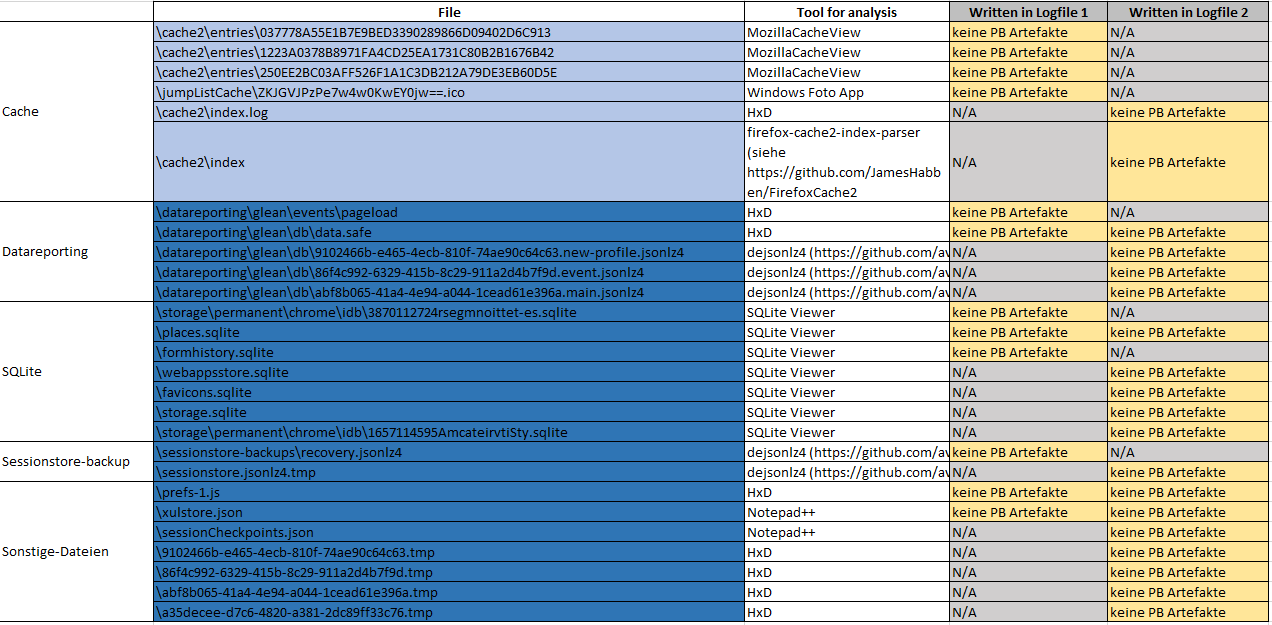
\includegraphics{bilder/firefox-tabelle-logfile1vlogfile2-reduced.png}}
%	\label{...}
	\caption{Tabelle mit wiederherstellbaren Dateien: Logfile 1 vs. Logfile 2}
\end{figure}

Allgemein: Artefakte in zwei "Common Pfaden"
-	(Local) %C:\Users\Forensik\AppData\Local\Mozilla\Firefox\Profiles\<Profile>.default-release\
-	(Roaming) %C:\Users\Forensik\AppData\Roaming\Mozilla\Firefox\Profiles\<Profile>.default-release\

Kategorien der Logs:
- Cache: 
	Logfile 1:
		> % \cache2\entries\037778A55E1B7E9BED3390289866D09402D6C913 (Local)
		> % \cache2\entries\1223A0378B8971FA4CD25EA1731C80B2B1676B42 (Local)
		> % \cache2\entries\250EE2BC03AFF526F1A1C3DB212A79DE3EB60D5E (Local)
		Analyse:
			- Tool: MozillaCacheView
			- TODO: Screenshot
		> % \jumpListCache\ZKJGVJPzPe7w4w0KwEY0jw==.ico (Local)
			- Tool: Windows Foto App
			- Enthält kleines "m" Icon
	Logfile 2:
		> % \cache2\index (Local)
		> % \cache2\index.log (Local)
		Analyse:
			- Tool: siehe Github und HxD
- datareporting:
	Logfile 1:
		> % \datareporting\glean\events\pageload (Roaming)
		> % \datareporting\glean\db\data.safe (Roaming)	
		Analyse:
			- Tool: HxD
			- keine PB Artefakte
	Logfile 2:
		*> % \datareporting\glean\db\data.safe (Roaming)
		> %  \datareporting\glean\db\9102466b-e465-4ecb-810f-74ae90c64c63.new-profile.jsonlz4 (Roaming)
		> % \datareporting\glean\db\86f4c992-6329-415b-8c29-911a2d4b7f9d.event.jsonlz4 (Roaming)
		> % \datareporting\glean\db\abf8b065-41a4-4e94-a044-1cead61e396a.main.jsonlz4 (Roaming)
		Analyse:
			- TODO: Definition glean
			- jsonlz4 Dateien (TODO: Definition) mit dejsonlz4 dekomprimiert (Quelle Github)
			- Dateien enthalten Systeminformationen im Json-Format (Screenshot?)
			- keine PB Artefakte
- Sessionstore-Backup:
	Logfile 1:
		> % \sessionstore-backups\recovery.jsonlz4 (Roaming)
		Analyse:
			- TODO: Definition sessionstore-backup = Datei, die Backup von Sitzungsdaten enthält
			- jsolz4 Datei in sessionstore-backup lassen sich mit Online-Tool parsen (https://www.jeffersonscher.com/ffu/scrounger.html)
			- Ergebnise: 
				Tab 1:  Willkommen bei Firefox [6.5.2023, 22:25:06, about:welcome;
				Tab 2:  Firefox Datenschutzhinweis — Mozilla [6.5.2023, 22:24:59], % https://www.mozilla.org/de/privacy/firefox/
			- Sind Seiten, die sich automatisch geöffnet haben, nachdem Firefox zum ersten Mal geöffnet wurde
			- keine PB Artefakte
	Logfile 2:
		> % \sessionstore.jsonlz4
		Analyse:
			- Lässt sich nicht mit Online-Tool aus Logfile 1 parsen
			- Stattdessen: dejsonlz4, danach Notepad++ mit JSON Plugin
			- Ergebnis: image-Eintrag als base64 entdeckt, in PNG umgewandelt (https://base64.guru/converter/decode/image), mit Windows Foto-App: "m" Icon (Mozilla-Logo)
- Sonstige Dateien:
	Logfile 1:
		> % \prefs-1.js
		> % \xulstore.json			
	Logfile 2:
		*> % \prefs-1.js (Roaming)
		*> % \xulstore.json (Roaming)
		> % \sessionCheckpoints.json (Roaming)
		> % \9102466b-e465-4ecb-810f-74ae90c64c63.tmp (Roaming)
		> % \86f4c992-6329-415b-8c29-911a2d4b7f9d.tmp (Roaming)
		> % \abf8b065-41a4-4e94-a044-1cead61e396a.tmp (Roaming)
		> % \a35decee-d7c6-4820-a381-2dc89ff33c76.tmp (Roaming)
	Analyse:
		- Weder JSON-Dateien (Notepad++) noch .tmp Dateien (HxD) enthalten PB Artefakte
		
- SQLite: (TODO: Abgleich mit Diffs-Exceltabelle, ob wirklich nur in places.sqlite geschrieben wurde)
	Dateien haben Sonderstellung:
		- Diese DBs dienen zur Verwaltung und Speicherung sämtlicher Browser Artefakte, insb. der Browser Historie
		- Aus diesem Grund: Dateien intensiver betrachtet
	Siehe Kapitel Methodik:
		> Entwicklung von Dateiinhalt in allen Snapshots (1, 2, 3 und 4) betrachtet
		> Für jeden Snapshot: 
			- SQLite-Datei extrahiert und mit SQLite-Datei aus vorherigem Snapshot verglichen
			- Untersuchung der SQLite-Dateien mit SQLite-Viewer (GUI-Tools)
			- Wenn zu SQLite-Datei WAL-Datei existiert: mit sqlite3 Kommandozeilentool PRAGMA wal\_checkpoint durchgeführt, danach neue SQLite-Datei mit ursprünglicher SQLite-Datei verglichen
		> Dabei gibt es drei Zustände: 
			- leere Datei
			- neuer (nicht-leerer) Inhalt
			- gleichbleibender Inhalt
	Mit Process Monitor Logfiles festgestellt, dass in folgende SQLite-DBs geschrieben: 
		(TODO: Tabelle mit Spalten: Dateiname, Zweck)
			Dateiename:							Zweck:
		- places.sqlite 						Browsing Historie
		- cookies.sqlite						Speichert Webseiten-Cookies
		- storage.sqlite						Speicher für Webseiten
		- favicons.sqlite						Speichert Icons für Lesezeichen
		- webappsstore.sqlite					Speicher für Webseiten
		- formhistory.sqlite					???
		- 1657114595AmcateirvtiSty.sqlite		> IndexedDB-Dateien, sind DBs, die von besuchten Webseiten
												angelegt werden % (https://www.reddit.com/r/firefox/comments/dri650/what_are_the_idb_files_in_the_permanent_storage/)
												> Im Chrome-Ordner: "the databases in the chrome subfolder relate to various pieces of integrated firefox functionality (content for the new tab page, blocklists, shield/normandy, remote settings, push api, ...)"
												> Enthalten eigentlich URL im Dateinamen
												> TODO: können geparsed werden: % https://stackoverflow.com/a/59923297/18037004
												"Activity Stream for Firefox is a collection of all the things you do in the browser that you care about displayed in a rich and meaningful way" 
												%https://wiki.mozilla.org/Firefox/Activity_Stream
												--> DB enthält keine Browsing Artefakte
		- 3870112724rsegmnoittet-es.sqlite		???
		
	Ergebnisse:
		\begin{figure}[h!]
			\centerline{\resizebox{\linewidth}{!}{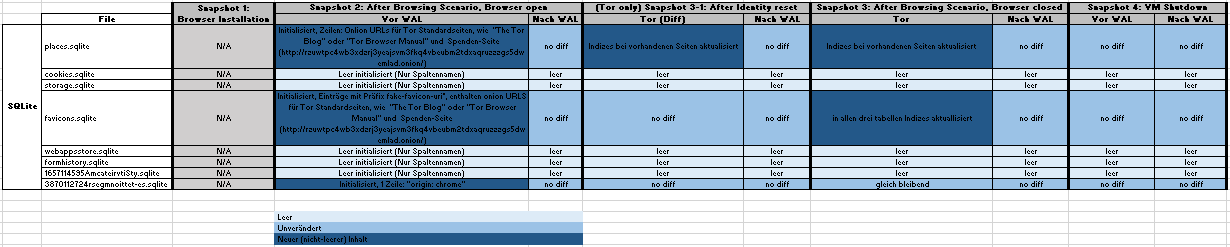
\includegraphics{bilder/tor-sqlite-table.png}}}
			\label{chart:final-criteria}  
			\caption{Comparison of found PB artifacts between RAM Dumps}
		\end{figure}
		> Nach Browser-Installation noch keine SQLite-Datei angelegt (Snapshot 1)
		> Während Browsing Szenario alle DBs Initialisiert, außer "webappsstore.sqlite" (Snapshot 2)
			- Dabei wurden in places.sqlite die Seiten geschrieben, die sich automatisch nach Browserstart im public Modus geöffnet haben (Datenschutzhinweise zu Firefox)
			- Restliche Dateien ohne Inhalt, nur Spaltennamen
			- Nach WAL Checkpoints bleiben Dateien unverändert
		> Nach Schließen des Browsers (Snapshot 3)
			- in places.sqlite: Indizes bei eingetragenen Seiten aktualisiert
			- 1657114595AmcateirvtiSty.sqlite erhielt BLOB Eintrag, in HxD keine Muster erkennbar
			- webappsstore.sqlite: leer initialisiert, nur Spaltennamen
			- restliche Dateien unverändert
			- nach WAL Checkpoints bleiben Dateien unverändert
		> Nach herunterfahren der VM (Snapshot 4)
			- Alle Dateien unverändert, auch nach WAL Checkpoint
	
- Zusammenfassung: in keiner Datei PB Artefakte


Quantitativ: (Diagramme)		
	> Balkendiagramm: Für jede Logfilekategorie: Anzahl Schreiboperationen Logfile 1 vs Logfile 2
	\begin{figure}[h!]
		\centerline{\resizebox{\linewidth}{!}{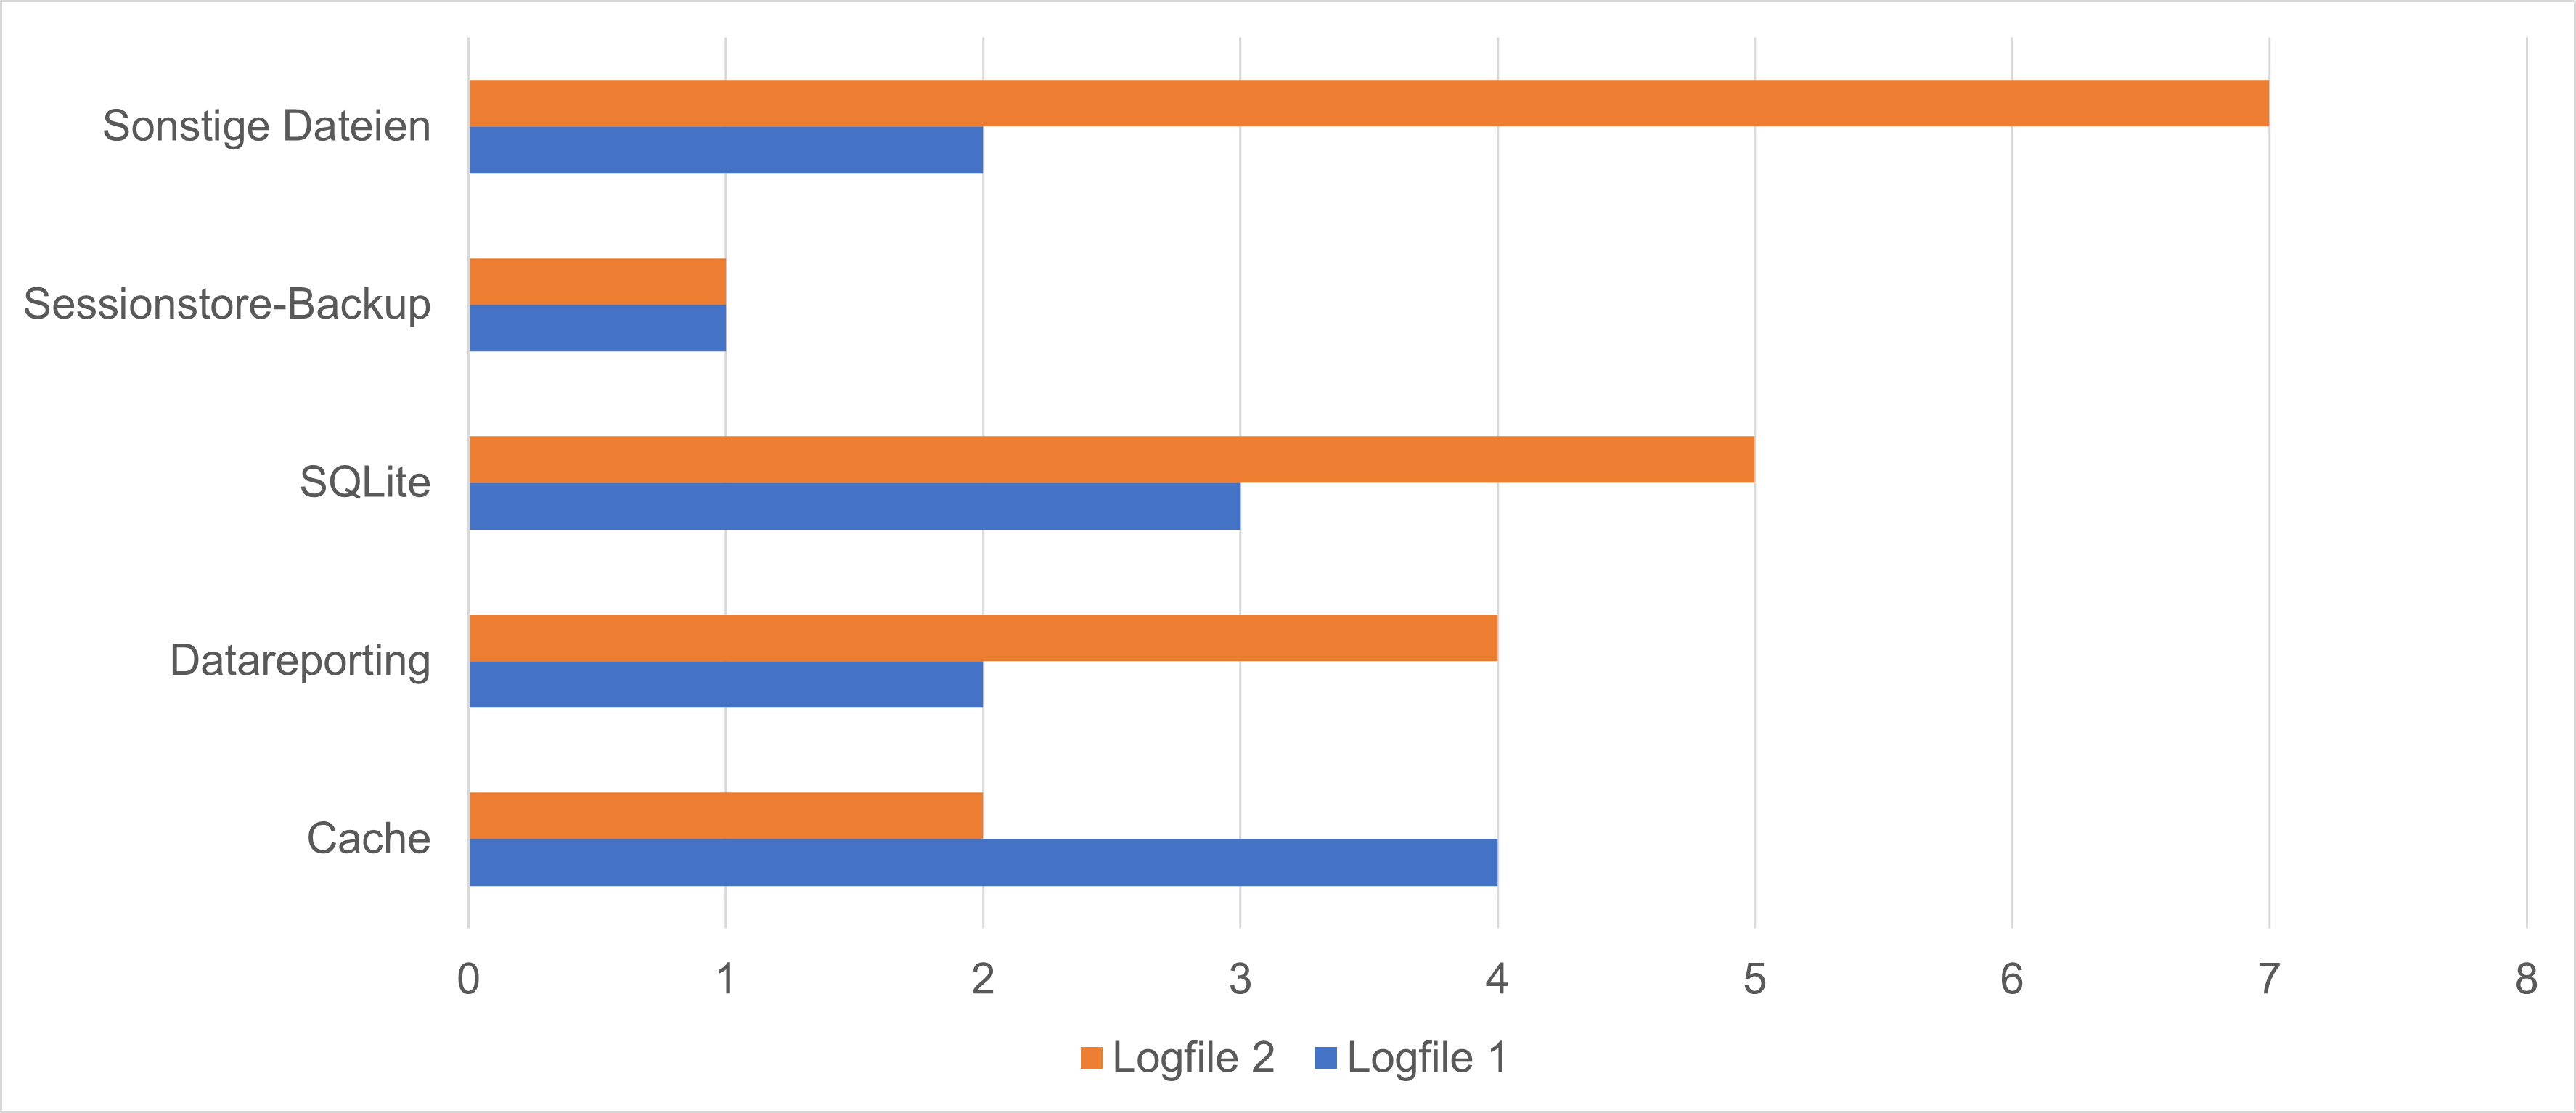
\includegraphics{bilder/bar-chart-logfile1vs2-test.png}}}
		\label{chart:final-criteria}  
		\caption{Comparison of found PB artifacts between RAM Dumps}
	\end{figure}

%Literatur:
%	o no traces were found in “common locations” \cite{Montasari.2015}
%		>  “places.sqlite”, “webappsstore. sqlite”, “sessionstore.bak”, “search.json” and “nssckbi.dll”
%	o	Safebrowsing: Alle Dateien in /safebrowsing-updating/ nicht relevant. Dort nur .vlpset und .sbstore Dateien. Speichern 256-Bit Hash von URLs, die auf SafeSearch Blacklist stehen 
%	o	Cache-Dateien: drei Caches: startupCache, jumpListCache (beide enthalten Binärdateien ohne Browsing Artefakte) und cache2 (können mit MozillaCacheView untersucht werden, enthalten keine Browsing Artefakte)
%	o	SQLite Datenbanken: Sqlite Dateien erst ohne WAL Dateien untersuchen, Danach mit sqlite3 Konsole: WAL in Datenbank schreiben mit: PRAGMA wal\_checkpoint; places.sqlite besonders relevant, da dort Browser in public Modus Browsing URLs verwaltet (Am besten hier vergleich mit Public Browsing machen)	
%		> \cite{Fayyad.2021} for Mozilla Firefox, 7 database files were recovered: cookies.sqlite-shm, places.sqlite-shm, prefs.js etc.
%		> \cite{Muir.2019} The two SQLite databases used by Firefox to track cookies and history (cookies.sqlite und places.sqlite) were both recoverable from the file system after deletion	
%		Ergebnisse stehen im Gegensatz zu \cite{Hedberg.2013} :
%			o	Chrome und Firefox: Einträge in places.sqlite + history.sqlite DB gefunden während PB! (Noch aktuell??)
%		Sonderfall: SQlite DB-Crash \cite{Hedberg.2013}
%			> WAL Files/Journal Files bei Crash gefunden -> Kann genutzt werden um zu beweisen, dass privater Browser genutzt wurde
%			> Daher: WAL Rollback mit sqlite3	
%	o	Jsonlz4 \& balkz4: Enthalten komprimierte Firefox-Sessions, jsonlz4 Dateien können mit Tool "entkomprimiert" werden: https://www.jeffersonscher.com/ffu/scrounger.html


\subsection*{Registry}
> Process Monitor: SetValue Operationen von Browser 
TODO: Logfile 1 vs 2?
	Kategorien Registry Keys:
	1) PreXULSkeletonUISettings:
		> Prefix: Absoluter Installationspfad von Firefox
		> Skeleton UI Einstellungen von Firefox % https://itigic.com/skeleton-ui-new-firefox-interface-to-start-up-much-faster/#google_vignette
			Definition:
				> Der "PreXULSkeletonUISettings" Registry Key enthielt Einstellungen für die Benutzeroberfläche (UI) des Firefox-Browsers, insbesondere für das sogenannte "Skeleton UI". Das Skeleton UI ist eine vereinfachte Benutzeroberfläche, die während des Ladens des Browsers angezeigt wird, bevor die vollständige Benutzeroberfläche geladen ist. Es besteht aus grundlegenden Steuerelementen und Elementen, die dem Benutzer die Interaktion ermöglichen, während der Rest der Benutzeroberfläche noch geladen wird.
				> Der "PreXULSkeletonUISettings"-Schlüssel enthielt Konfigurationsoptionen wie Farben, Positionen und andere Einstellungen für das Skeleton UI. Durch das Bearbeiten dieses Schlüssels konnten Benutzer die Darstellung des Skeleton UI anpassen. Es ist jedoch wichtig zu beachten, dass das Ändern der Registrierungseinträge ein fortgeschrittenes Verfahren ist und Fehler zu Problemen mit dem Browser führen kann.
			
		> Struktur der Keys: % HKCU\SOFTWARE\Mozilla\Firefox\PreXULSkeletonUISettings\C:\Program Files\Mozilla Firefox\firefox.exe|<UI Einstellung>
		> Unterschiedliche UI Einstellungen
			- % ScreenX (DWORD)
			- % ScreenY (DWORD)
			- % Width (DWORD)
			- % Height (DWORD)
			- % Maximized (DWORD)
			- % Flags (DWORD)
			- % CssToDevPixelScaling (REG_BINARY)
			- % UrlbarCSSSpan (REG_BINARY)
			- % SearchbarCSSSpan (REG_BINARY)
			- % SpringsCSSSpan (REG_BINARY)
		> keine PB Artefakte unter UI Einstellungen	
	2) Business Activity Monitoring % https://learn.microsoft.com/de-de/biztalk/core/business-activity-monitoring-bam
		> Quelle: % https://notes.qazeer.io/dfir/windows/_artefacts_overview
		> BAM is a mostly undocumented feature that controls the programs executed in the background. DAM is a feature for devices supporting the "Connected Standby" mode (i.e when a device is turned on, but its display will be turned off). As a result, the BAM registry keys will contain data on any devices, while DAM registry keys will only contain data on mobile devices.
		> The BAM registry key contains multiple subkeys under bam\\State\\UserSettings, with one subkey per user, identified with the user SID. While the key is in the SYSTEM registry hive, program executions can thus still be tied to a specific user using this SID.
		> Each user-specific key contains a list of executed programs, with their full path and timestamp of last execution.
		> If a file is deleted, the eventual associated entry in the BAM is deleted as well after the system reboot. Additionally, BAM entries older than 7 days are deleted upon system boot. The BAM thus provides limited information on historic execution of programs
		> No entries are created in the BAM keys for executables on removable media and/or on network shares.
		> Key: %  HKLM\System\CurrentControlSet\Services\bam\State\UserSettings\S-1-5-21-588412547-2749917301-3803556669-1001\\Device\HarddiskVolume2\Program Files\Mozilla Firefox\firefox.exe (REG_BINARY)

Quantitativ: (Diagramme)
	- Stacked Balkendiagramm jeweils für Logfile 1 und Logfile2: Anteil Kategorie 1 bzw.2 an allen Registry-Schreiboperationen
	\begin{figure}[h!]
		\centerline{\resizebox{\linewidth}{!}{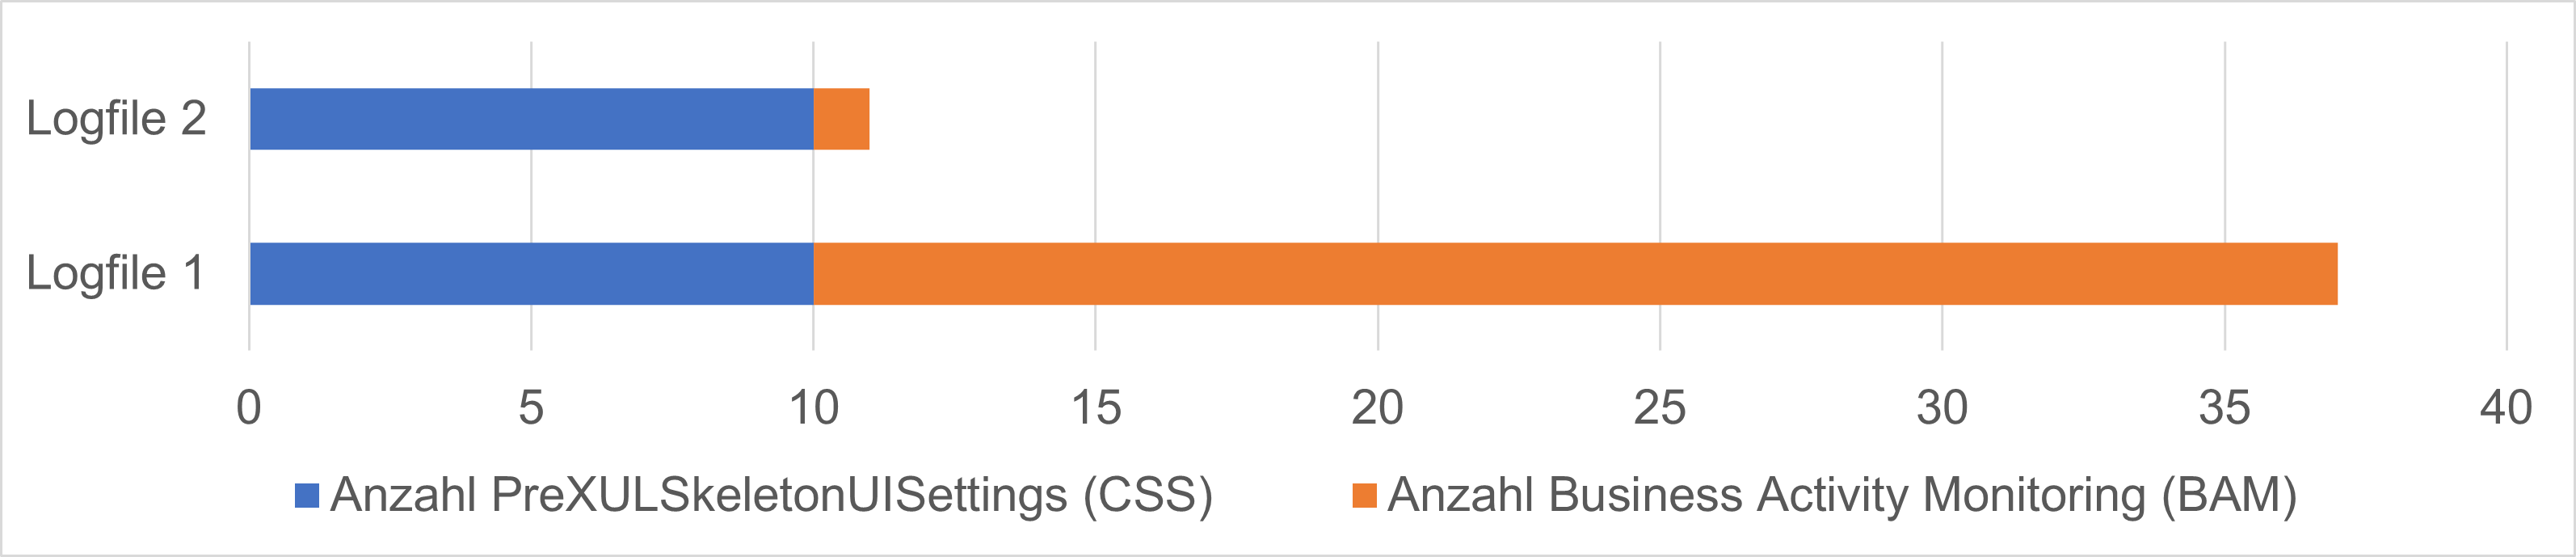
\includegraphics{bilder/firefox-registry-stacked-bar-chart.png}}}
		\label{chart:final-criteria}  
		\caption{Comparison of found PB artifacts between RAM Dumps}
	\end{figure}
	
> Stringsuche in Registry Hives mit Registry Explorer (Siehe Liste)
	In allen Hives kein Treffer für alle Suchbegriffe

Literatur: 
	> angeblich in Shellactivities Ergebnisse. --> Nicht mehr vorhanden in aktueller Version (Verweis auf E-Mail)

%Literatur:
%	>	Auf Autor verweisen: angeblich in Shellactivities Ergebnisse. --> Nicht mehr vorhanden in aktueller Version (Verweis auf E-Mail)
%	>	Process Monitor/Regshot zeigen keine relevanten Key-Änderungen
%	> \cite{Muir.2019}: Autopsy Keyword Suche nach Suchbegriffen: Ergebnisse in \%SystemRoot\%Minidump NTUSER.DAT, ntuser.dat.LOG1 (a log of changes to NTUSER.DAT)
%	> Zentral: shellactivites Key:	NTUSER.DAT --> “shellactivities” key \cite{Muir.2019}
%	> \cite{Rochmadi.2017} Detection of registry changes helps to determine what the appropriate plugin is used to search for digital evidence using volatility memory forensic:
%	- RegQueryValue:	HKCU/Software/Microsoft/Windows/CurrentVersion/InternetSettings/Connections/DefaultConnectionSettings
%	- RegCloseValue: 	HKCU/Software/Microsoft/Windows/CurrentVersion/InternetSettings/Connections
%	- IRP\_MJ\_READ: C:/pagefile.sys

\subsection*{Black-Box Analyse/Uncommon Locations}

\subsubsection*{Analyse mit Autopsy}
Bei White-Box Analyse/Common Locations: Autopsy nur zur Dateiextraktion genutzt, hier: als konkretes forensisches Werkzeug

Stichwortsuche:
- In allen Snapshots keine Treffer (auch innerhalb \$Carved)
- TODO: Pagefile gefunden?

Von Autopsy automatisch indexierte Dateien: 
In allen Fällen: keine Dateien gelöscht, nur über Zeitraum der Snapshots neue dazugekommen
- Web Bookmarks:
	\begin{figure}[h!]
		\centerline{\resizebox{\linewidth}{!}{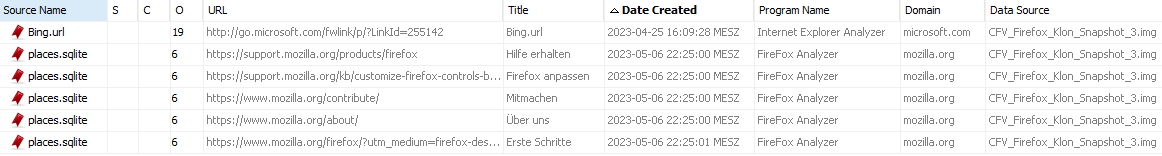
\includegraphics{bilder/cfv_firefox_autopsy_web_bookmarks.png}}}
		\label{chart:final-criteria}  
		\caption{Autopsy Web Bookmarks}
	\end{figure}
	Snapshot 1:
		> Bing.url (Unter C:/User/Forensik/Favorites/Links) enthält Bing Startseite
	Snapshot 2:
		> 5 Einträge in places.sqlite: (Firefox Standardseiten -> Deckt sich mit Beobachtungen aus Process Monitor Analyse, siehe Kapitel X)
	Snapshot 3:
		> unverändert zu 2
	Snapshot 4:
		> unverändert zu 3
- Web Cookies:
	\begin{figure}[h!]
		\centerline{\resizebox{\linewidth}{!}{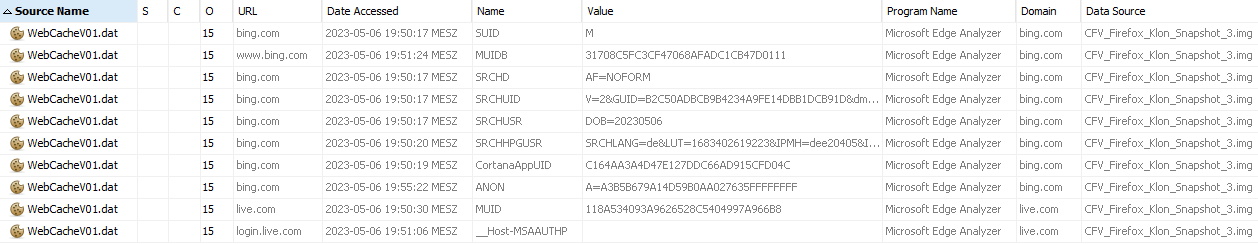
\includegraphics{bilder/cfv_firefox_autopsy_web_cookies.png}}}
		\label{chart:final-criteria}  
		\caption{Autopsy Web Cookies}
	\end{figure}
	Snapshot 1:
		> 10 Einträge in WebCacheV01.dat (= DB des Internet Explorers zum speichern von Browserdaten): Cookies für bing.com und live.com (= outlook)
	Snapshot 2:
		> unverändert zu 1
	Snapshot 3:
		> unverändert zu 2
	Snapshot 4:
		> unverändert zu 3
- Web History:
	\begin{figure}[h!]
		\centerline{\resizebox{\linewidth}{!}{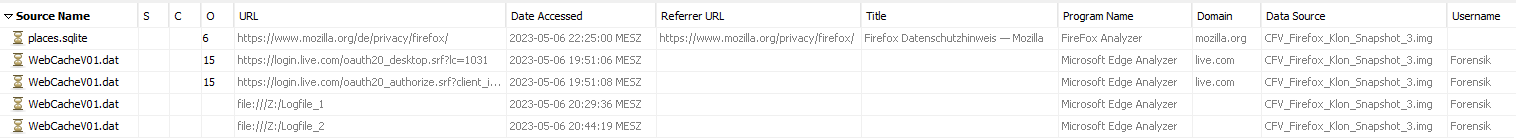
\includegraphics{bilder/cfv_firefox_autopsy_web_history.png}}}
		\label{chart:final-criteria}  
		\caption{Autopsy Web History}
	\end{figure}
	Snapshot 1:
		> 2 Einträge in WebCacheV01.dat:
			- 2x live.com (= outlook)
	Snapshot 2:
		> 1 Eintrag in places.sqlite: % https://www.mozilla.org/privacy/firefox/
			-> Zurückzuführen auf Seite, die sich automatisch geöffnet hat, als Firefox gestartet (bevor privates Fenster geöffnet wurde)
		> 1 neuer Einträge in WebCacheV01.dat:
			- file:///Z:/Logfile\_1 (= Process Monitor Logfile, die in shared-Folder geladen wurde) -> Erklärung?
	Snapshot 3:
		> 1 neuer Eintrag in WebCacheV01.dat:
			- file:///Z:/Logfile\_2 (= Process Monitor Logfile, die in shared-Folder geladen wurde) -> Erklärung?
	Snapshot 4:
		> unverändert zu 3
- Web Categories:
	\begin{figure}[h!]
		\centerline{\resizebox{\linewidth}{!}{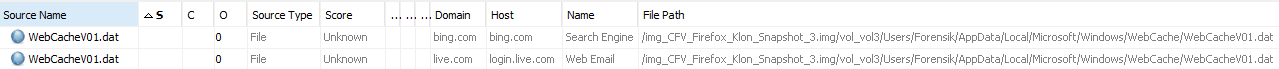
\includegraphics{bilder/cfv_firefox_autopsy_web_categories.png}}}
		\label{chart:final-criteria}  
		\caption{Autopsy Web Categories}
	\end{figure}
	Snapshot 1:
		> 2x WebCacheV01.dat aufgelistet => Mit HxD untersucht, keine PB Artefakte
	Snapshot 2:
		> unverändert zu 2
	Snapshot 3:
		> unverändert zu 3
	Snapshot 4:
		> unverändert zu 4
		
Zusammenfassung:
- keine PB Artefakte
- Keine neuen Erkenntnisse vgl. mit intensiver Analyse mittels Process Monitor in Kapitel X
- Eintrag von Datenschutzseite in places.sqlite wurde erkannt.

%Literatur:
%	o	Autopsy Keywortsuche: 
%		>	In alles Snapshots ergebnislos (keine Keyword-Hits
%		-->	In Literatur: Autoren fanden Ergebnisse in pagefile.sys 
%			> Autopsy: websites and some of the keywords found in hidden file called “pagefile.sys” \cite{Mahlous.2020}
%			o \cite{Montasari.2015} traces were found in: 
%				> However, on investigating the “pagefile.sys”, some entries were discovered
%				> Using the “data carving” technique, profile picture was recovered
%			o \cite{Said.2011} 
%				> Examining pagefile.sys showed some positive hits 			
%		--> Evtl. hier zeigen, was gefunden werden kann, wenn RAM reduziert
%		--> Aber auf Problem hinweisen, dass gefundener String in pagefile nicht direkt Browser zugeordnet werden kann
%		> \cite{Gabet.2018}	Firefox only produced three recoverable artefacts as reported by both tools (FTK, Autopsy) --> Artefakte werden nicht genannt!
%		> \cite{Muir.2019} Autopsy Keyword Suche nach Suchbegriffen: unallocated space
%		> Autopsy Carving Module (\$Carved): \cite{Muir.2019}
%			•	When searching for the string ’clot’ from the browsing protocol, six .dll, .edb and .reg files were discovered in unallocated space.
%			•	Further searching of unallocated space uncovered references to the Tor installation directory and the obfs4 bridging IP addresses
%			•	browsing data found in NTUSER.DAT was also replicated in unallocated space.
%	o	Autopsy PlugIns:
%		>	*** TODO: Hier Liste mit PlugIns ***

\subsubsection*{Analyse mit Volatility}
Vorgehen: Siehe "Methodik" Kapitel
	- Ausgangslage: Volatility Yarascan Treffer
	- Für jeden Treffer: virtueller Offset des Strings, PID, getriggerte Yararule, getriggerte Yara Component z(= Variablenname des gesuchten Strings), gefundener String
	- Neue Spalte: "Prozessname" -> zu jeder PID Prozessnamen
	- Ergebnisse Aufbereitet nach folgendem Schema:
		> Für jeden RAM Dump
		> Für jede Yararule
		> Für jede Component
		> Filter: Prozessname = Firefox -> Anzahl zählen
		> Filter: Prozessname = Alle Prozesse außer Firefox -> Anzahl zählen

Yararule "Keyword":
	\begin{figure}[h!]
		\centerline{\resizebox{\linewidth}{!}{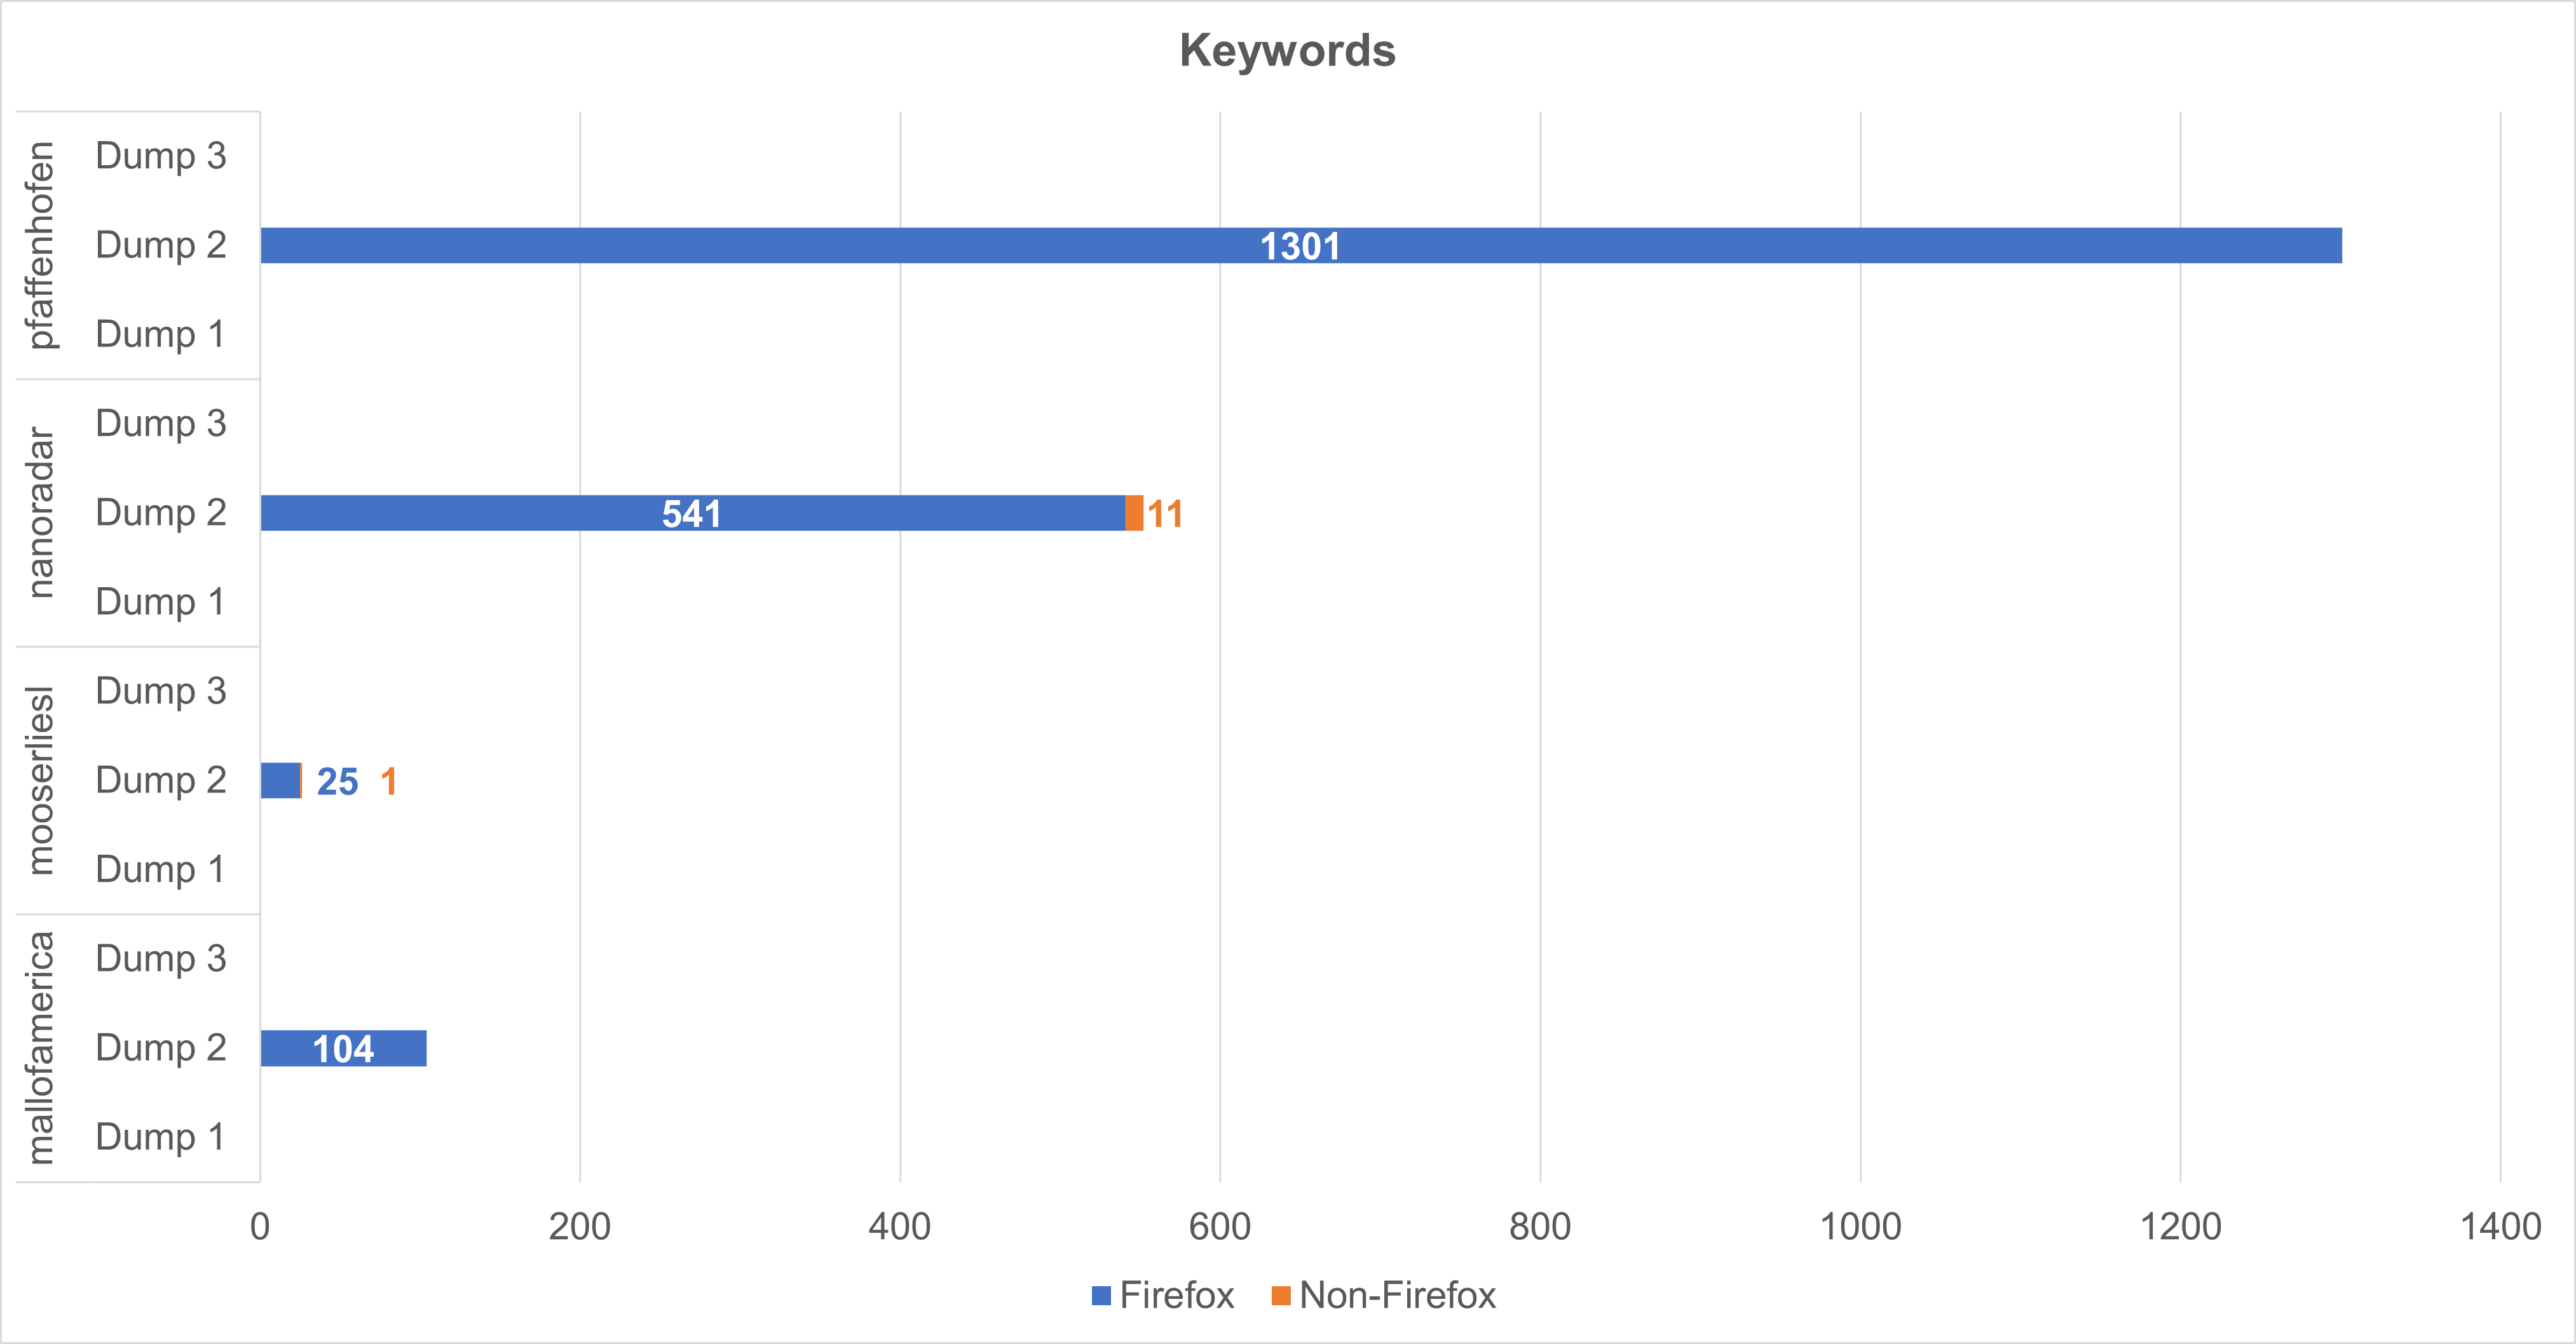
\includegraphics{bilder/volatility/firefox/keywords.png}}}
		\label{chart:final-criteria}  
		\caption{Keywords}
	\end{figure}
	Analyse:
		> Ausschließlich in RAM Dump 2 Keyword Artefakte gefunden
		> Hauptsächlich in Firefox Prozess
		> Mit 1301 Artefakten, am häufigsten pfaffenhofen vertreten. Vermutung: Evtl. weil Google Maps viele zusätzliche Artefakte lädt. 
		
Yararule "URL":
	\begin{figure}[h!]
		\centerline{\resizebox{\linewidth}{!}{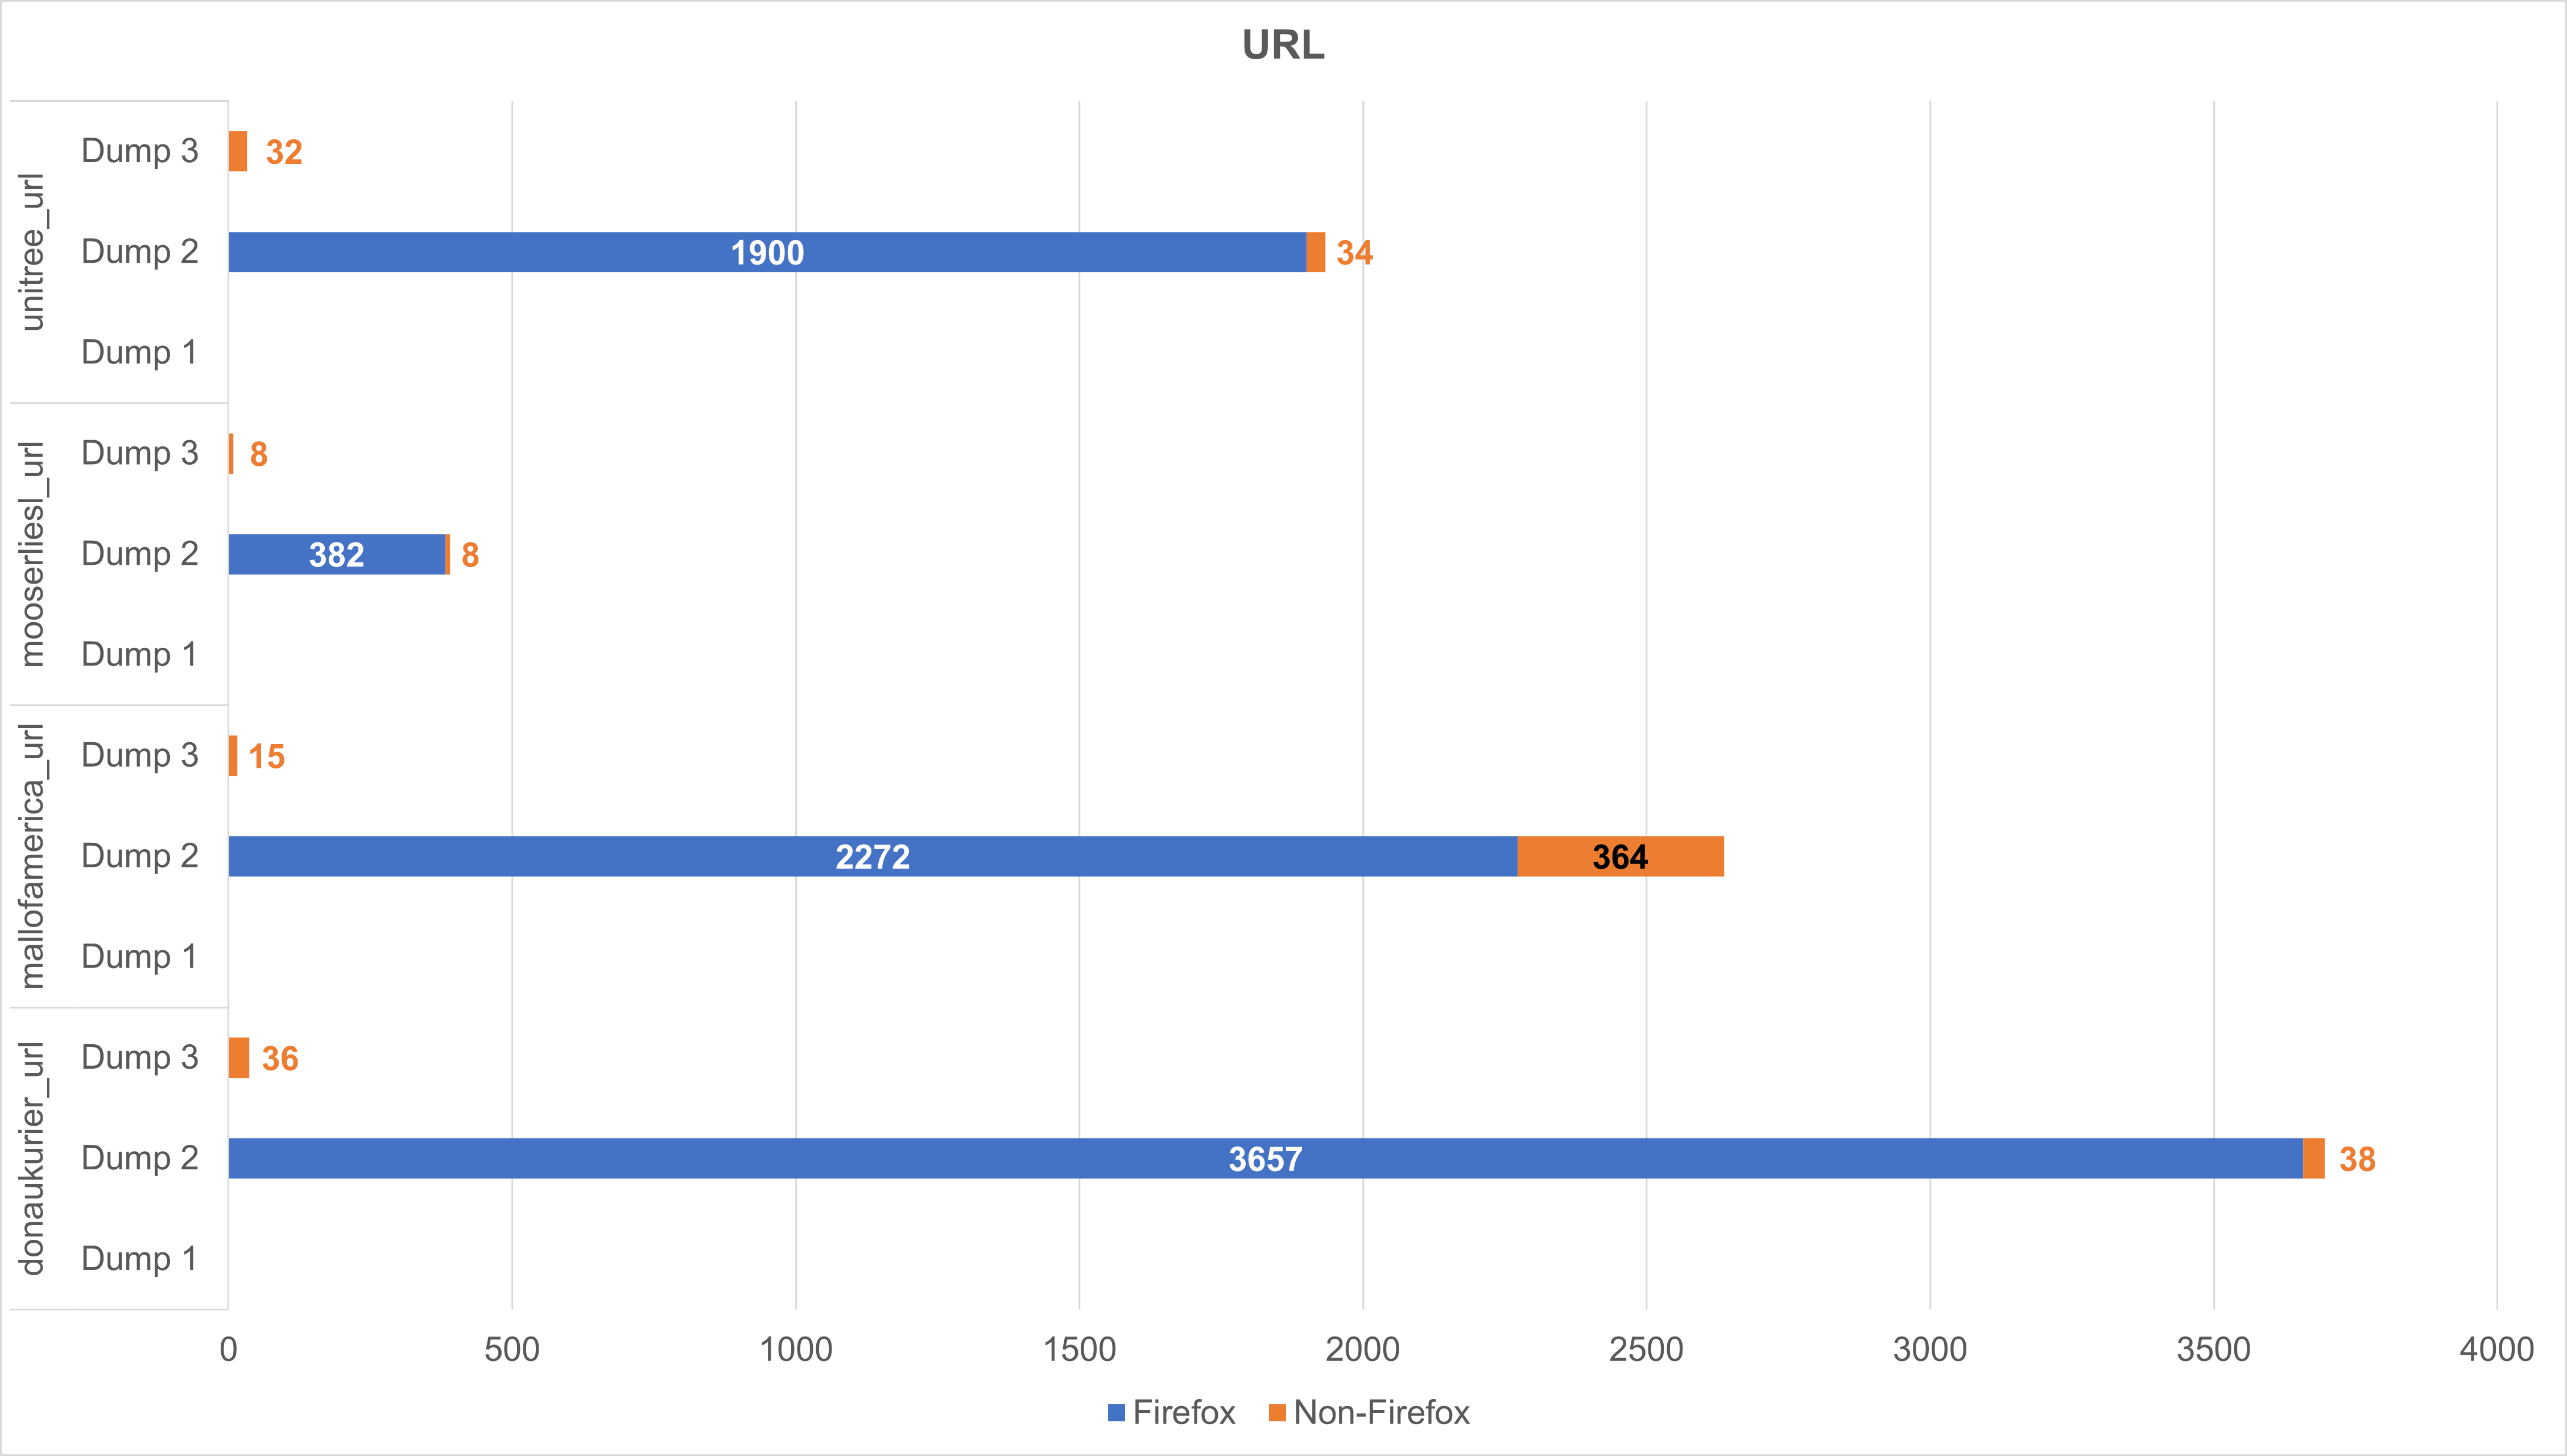
\includegraphics{bilder/volatility/firefox/url.png}}}
		\label{chart:final-criteria}  
		\caption{URL}
	\end{figure}
	Analyse:
		> Wie bei anderen Kategorien: Die meisten Artefakte in RAM Dump 2, in Firefox Prozessen
		> mooserliesl tritt am wenigsten auf, donaukurier am meisten (vmtl. auf Öffnen von Bild zurückzuführen)
		> Hier bemerkenswert, dass in RAM Dump 3 Artefakte von allen vier URLs zu finden sind
		> Bei genauerer Analyse des Process Monitor Logfiles herausgefunden: Artefakte alle in svchost.exe Prozess gefunden
		> Deshalb RAM Dump erneut mit Volatility windows.svcscan Plugin untersucht:
			"The svcscan plugin allows the analyst to list out the services running. This plugin gives more detail to the running processes in the event that the analyst requires additional details such as the display name, binary path, or service type." % (https://www.oreilly.com/library/view/digital-forensics-and/9781787288683/9ab60586-2b04-45e0-b437-dbfe10ab3be8.xhtml)
		> Ausgabe aller im RAM gefundener Services
		> Problem: Volatility svcscan liefert keine PID zu laufenden Services
		> Deshalb: "White-Box" Analyse: Snapshot 3 erneut aufgetaut, danach mit Process Explorer PID X (TODO!) von SVChost Prozess gesucht, in dem PB Artefakte gefunden wurden
			Def. Process Explorer:
				"Prozess Explorer zeigt Ihnen Informationen darüber an, welche Handles und DLLs-Prozesse geöffnet oder geladen wurden." % https://learn.microsoft.com/de-de/sysinternals/downloads/process-explorer
				"Process Explorer, from Sysinternals, is a process management program that allows you to see the running processes on your computer and a great deal of information about each process. One of the nice features of Process Explorer is that it also gives you the ability to see what services a particular SVCHOST.EXE process is controlling."
		> Ergebnis: DNSCache Service mit PID X (TODO!) = DNScache Service
			TODO: Screenshot
		> Ausführung von ipconfig /displaydns liefert gecachte URLs
			TODO: Screenshot
		> Nach Löschen des DNSCaches mit ipconfig /flushdns + Schließen aller Process Monitor Instanzen + Beenden des DNSCaches Services + Erneuter RAM-Dump -> Keine PB Artefakte mehr gefunden!
Yararule "Mail":
	\begin{figure}[h!]
		\centerline{\resizebox{\linewidth}{!}{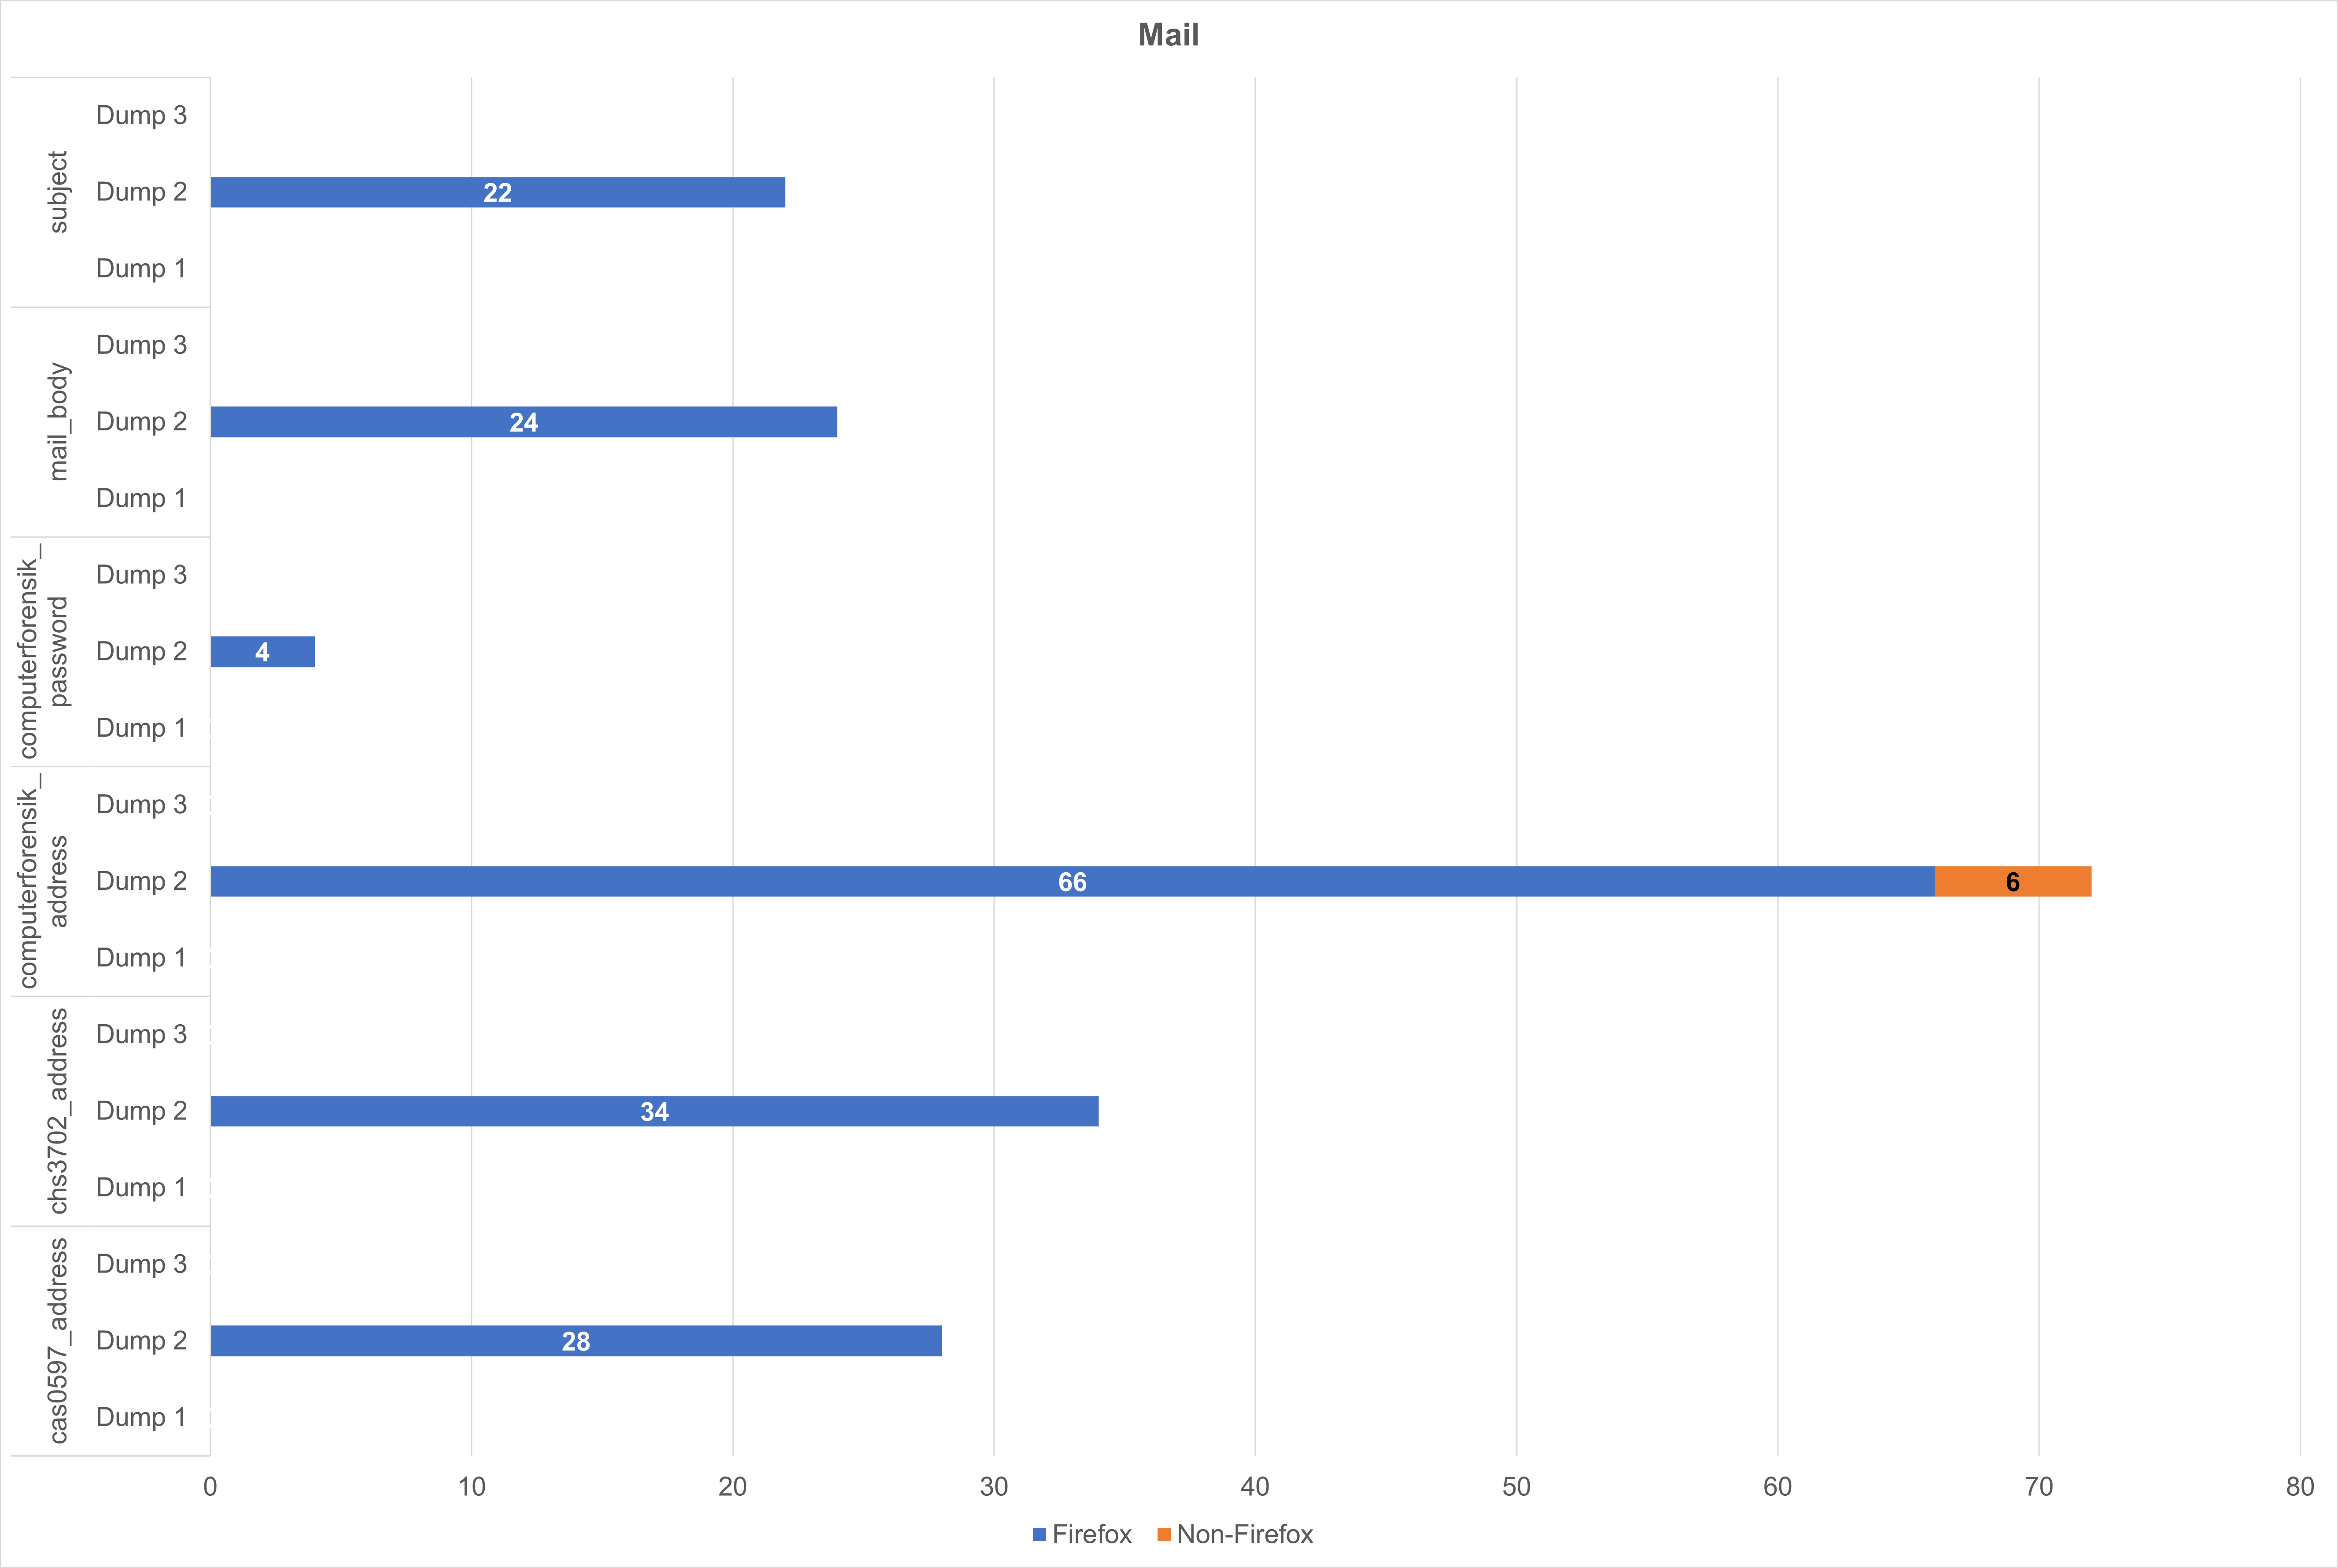
\includegraphics{bilder/volatility/firefox/mail.png}}}
		\label{chart:final-criteria}  
		\caption{Mail}
	\end{figure}
	Analyse:
		> Alle Mail Artefakte gefunden
		> Ausschließlich in RAM Dump 2 Mail Artefakte gefunden
		> Am häufigsten Absenderadresse "computerforensikvl@gmail.com" gefunden, als einziges Artefakt auch in anderen Prozessen gefunden.
		> Bemerkenswert: Passwort wurde 4x als Klartext im RAM gefunden!
			String Kontext:
				Offsets:		PIDs:
				0xb9ce29180c8	7420
				0x2859f4ffd4e0	7420
				0x24083b41858	8424
				0x240840e5b08	8424
				
Yararule "Image":
	\begin{figure}[h!]
		\centerline{\resizebox{\linewidth}{!}{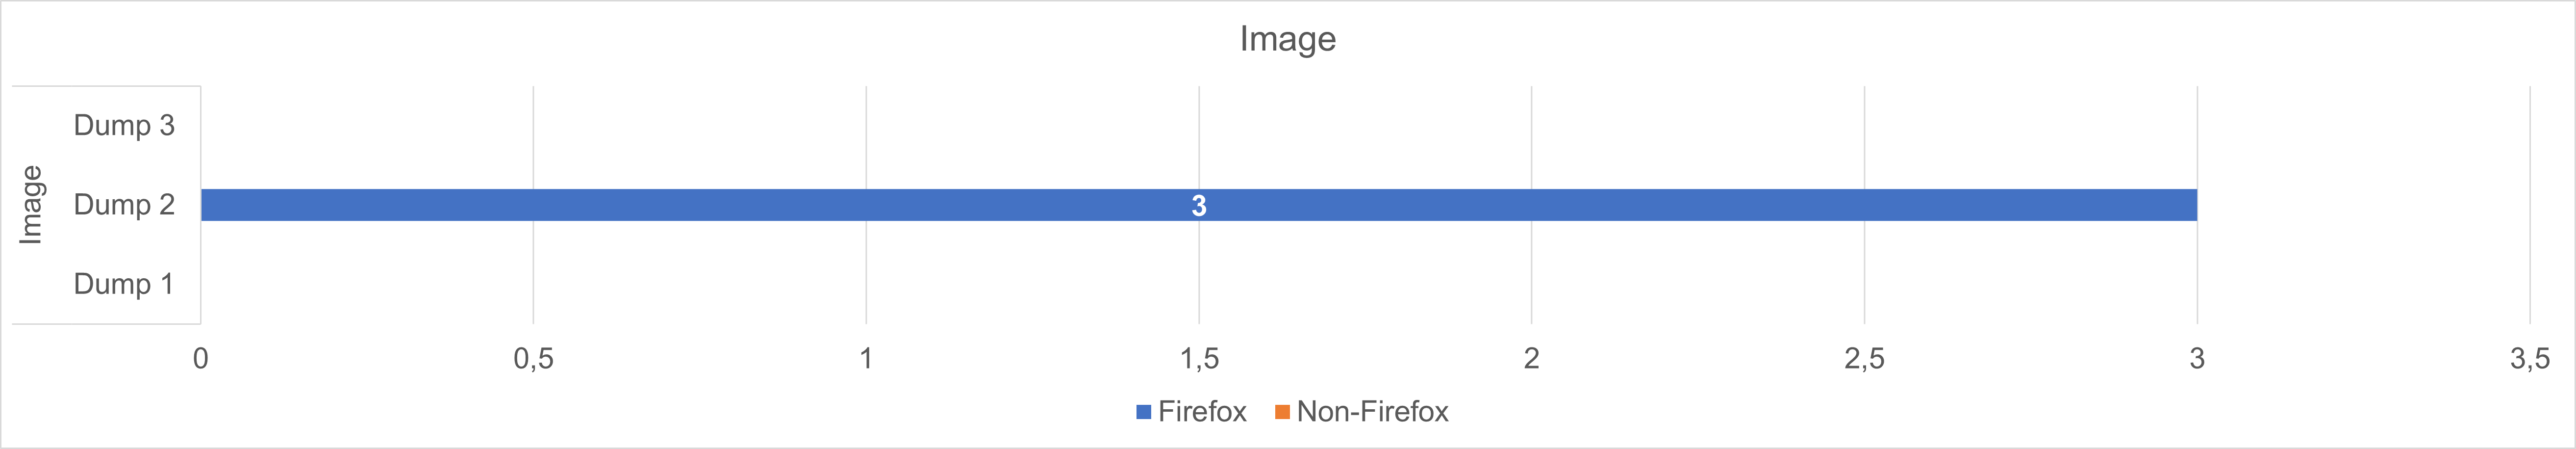
\includegraphics{bilder/volatility/firefox/image.png}}}
		\label{chart:final-criteria}  
		\caption{Image}
	\end{figure}
	Analyse:
		> Hex-Wert von Donaukurier Bild wurde im 2. RAM Dump in 3 Firefox Prozessen gefunden
	

Zusammenfassung = Stacked Bar Chart:
\begin{figure}[h!]
	\centerline{\resizebox{\linewidth}{!}{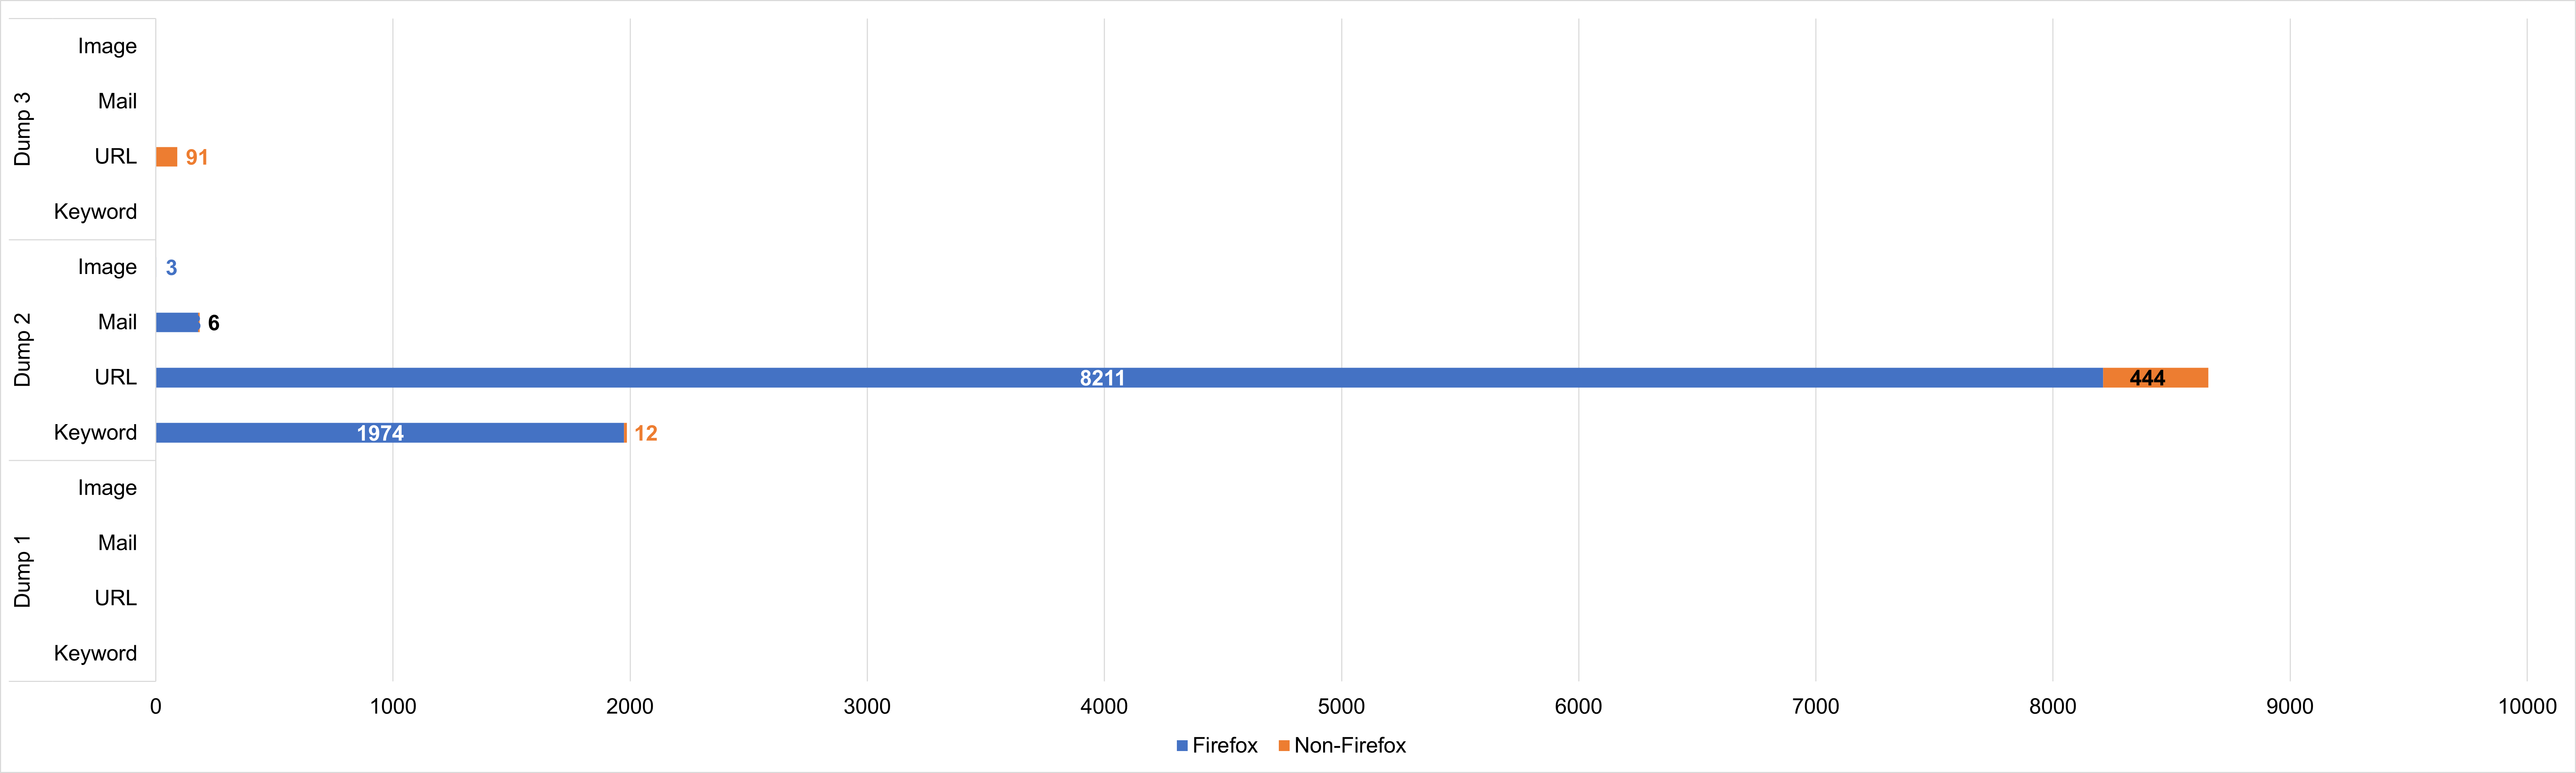
\includegraphics{bilder/volatility/firefox/summary.png}}}
	\label{chart:final-criteria}  
	\caption{Summary}
\end{figure}

TODO: Kreisdiagramme/Balkendiagramme mit Gesamtzahl an (Non-)Firefox Yarascan-Treffer erst im Vergleich mit Tor

\subsection*{Uncommon Locations}

Literatur:
%o Autopsy: \cite{Muir.2019}
%	•	Configuration files, downloaded files, and browserrelated data are recoverable from the file system.
%	•	Significant data-leakage from the browsing session occurred: HTTP header information, titles of web pages and an instance of a URL were found in registry files, system files, and unallocated space.
%o RAM-Analyse nach \cite{Muir.2019}:
%	•	Live-Analyse identifiziert auch nach dem Schließen und Deinstallieren des Browsers und Abmelden des Benutzers Spuren von Tor-Prozessen, einschließlich des absoluten Pfads zur Browser-Executable, des Benutzernamens und des Geräts, von dem es ausgeführt wurde.
%	•	The data-leakage contained the German word for ’search’ in reference to a Google search. This hints at the locale of the Tor server used to exit the network (exit relay).
%
%o RAM-Analyse nach \cite{Hariharan.2022}:
%	o	process was found to be firefox.exe
%	o	pslist and pstree: parent process was shown 
%	o	Belkasoft Ram Capturer: retrieve information about facebook
%	o	Cmdline: file path of the browser “E:/TorBrowser/Browser/firefox.exe” + name of process tor.exe and firefox.exe
%	o	Dlllist: DLL files of the executable files were not captured
%	o	Netscan: tor.exe + obfs4proxy.exe -> showed “LISTENING” connections to nonstandardized ports as output.
%	Yarascan: was able to retrieve all the browsing sessions
%o RAM-Analyse nach \cite{Sajan.2021} mit Volatility
%	•	process list extracted from the memory
%	•	registry hives been extracted from the memory dump
%	•	threads were extracted: “D:/VolatilityWorkbench/volatility.exe”–plugins=”D:/VolatilityWorkbench/profiles” pslistfilename =”C:/Users/username/Desktop/tor.raw” –profile=Win10x64 17763 –kdbg=0xf807606ac5e0
%	•	Handles: resources used by the process 5672
%	•	Dlls: These dlls can be found from prefetch file --> Can be found in “prefetch” file -> Analyzed with “winprefetchview”
%	•	Places.sqlite: SQLite viewer has been used to recover bookmarks and frequently visited sites even after uninstalling the application
%	•	Visited Websites: Using keyword search in Dump’s Hex
%
%o Registry:
%	> Shellactivites (siehe Firefox) \cite{Muir.2019}: instance of a URL were found in registry file
%	> \cite{Nelson.2020} The userassist key is located in the NTUSER.dat hive of the
%		 -> Registry and indicates the execution path of the program, as well as the number of times the program was executed 




\section{Chrome}

\subsection*{Uncommon Locations}

o Autopsy Keyword-Suche: 
	> Chrome and Edge produced five artefacts as reported by both tools. (FTK, Autopsy) \cite{Gabet.2018}
		--> Artefakte werden nicht genannt!
	> only two temporary files (Figure 7) were recovered with Minitool Power Data Recovery but it was a dead end; Location: appdata/…/Chrome/…/ Preferences/RF1533fa.TMP \cite{Fayyad.2021}
	> pagefile.sys file showed no traces at all \cite{Said.2011}
	

\section{Brave}